%!TEX root = ../thesis.tex
%*******************************************************************************
%*********************************** Fifth Chapter *****************************
%*******************************************************************************

\chapter{Correlated Principal Analysis through Conditional Expectation \label{cha:cpace}}  %Title of the Fifth Chapter

\ifpdf
    \graphicspath{{Chapter5/Figs/Raster/}{Chapter5/Figs/PDF/}{Chapter5/Figs/}}
\else
    \graphicspath{{Chapter5/Figs/Vector/}{Chapter5/Figs/}}
\fi

The foray into modelling using the spatial dimensions as the functional dimension in Chapter~\ref{cha:ftsm} gave us two clear findings.
Firstly, that spatial information is often useful in reconstruction and ignoring the spatial correlation observed between functional observations is throwing away information.
Secondly, smoothing across the spatial dimension can be problematic since it is incredibly easy to over smooth and lose important spatial details in the reconstructions. 
We note from Chapter~\ref{cha:ftsm} that the standard model, using time as the functional domain, managed to capture high levels of spatial detail since it treats each function as independent.
The downside to this model is that unobserved spatial locations cannot be reconstructed as we have no information about how to interpolate between functional observations.
One natural way to consider modelling such functional data is then to extend this model but to explicitly include the correlation between the observations in the model. 
We discuss these models in this chapter, we start with a discussion on models where the correlation between functional observations is purely spatial.

\section{Spatially Correlated Functional Data, \label{sec:space}}
The CESM-LE data set, as described in Chapter~\ref{cha:data}, provides a perfect example of spatially correlated functional data.
Take Figure~\ref{fig:cesm-space} for example, which shows the functional observations of the reference height temperature at 6 locations; the United Kingdom (UK), Ireland (IE), France (FR), Colombia (CO), Venezuela (VE), and Ecuador (EC). 

 \begin{figure}[htbp!] 
	\centering    
	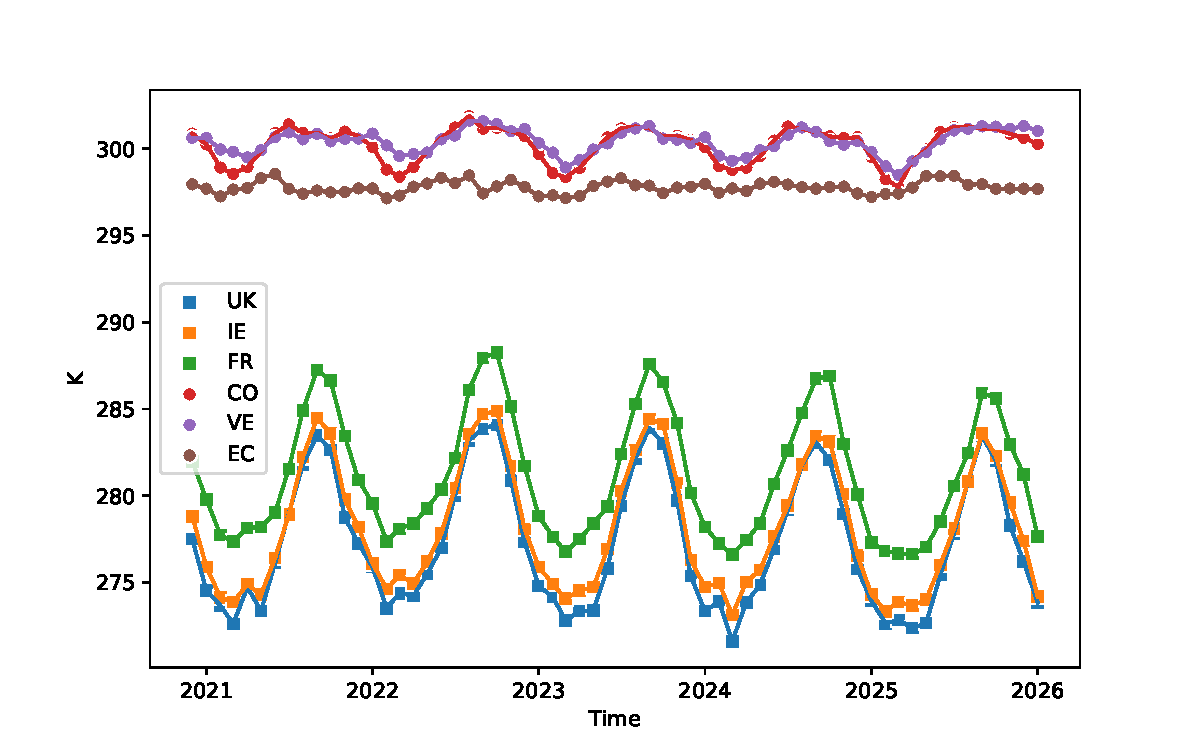
\includegraphics[width=1.0\textwidth]{TREFHT_example_space_temp}
	\caption[An example of spatial correlation in the TREFHT variable from the CESM-LE dataset.]{Example of functional observations reference height temperature across the globe from the CESM-LE dataset. Notice that clearly locations close to each other in the globe tend to have more similar structure.}
	\label{fig:cesm-space}
\end{figure}
Clearly we can see locations in a similar vicinity having similar temperature patterns.
The European countries have a much larger range and overall lower mean temperature than those of the South American countries.
However, there are some similarities between all countries, such as the periodic nature of the functions, which indicate that there is some share of information across even large spatial distances. 

Incorporating spatial information into the models such as PACE, described in Section~\ref{sec:pace}, is therefore a natural extension. 
One such approach to this has been considered by \citeauthor{liu_functional_2017} in \citep{liu_functional_2017}. 
We will describe their model below and use this as our basis for modification and expansion in our proposed model for correlated functional data.

\subsection{Spatial principal analysis through conditional expectation, \citep{liu_functional_2017}, \label{ssec:space}}
A natural way to incorporate spatial correlation in our functional observation from the PACE model is to adjust how we define the score processes in Equation~\eqref{eqn:fd_temporal_fpca}.
The PACE model, \citep{yao_functional_2005}, implicitly uses the fact that $\mathbb{E}\left(\xi_{ik} \xi_{jk}\right) = 0$ for $i \ne j$ and $k=1,2,\cdots,K$. 
The Spatial PACE model (SPACE), \citep{liu_functional_2017} explicitly incorporates a model for this covariance.
In particular they consider the following form:
\begin{equation}
	\text{Cov}\left(\xi_{ip}, \xi_{jq}\right) = \begin{cases}
		\lambda_k \rho_{ijk}\text{ for $p=q=k$.} \\
		0 \text{ otherwise.}
	\end{cases}
\label{eqn:space_score}
\end{equation}
where $0 \le i, j \le N$ index the functional realisation and $0 \le p, q \le K$ index the component.
The correlation is induced by specifying the form of $\rho_{ijk}$ which acts as a spatial correlation factor in \citep{liu_functional_2017}. 
As such, it is useful to explicitly describe the association by writing $\rho_{ijk} = \rho_{k} \left( \vesub{s}{i}, \vesub{s}{j} \right)$ where $\ve{s}$ is an element in the spatial domain $\mathcal{S}$ as discussed in Chapter~\ref{cha:Into}.
Often the correlation structure may have an assumed parametric form, in which case we write $\rho_k \left(\ve{s}, \ve{s}^\prime \right) = \rho_k \left(\ve{s}, \ve{s}^\prime; \ve{\theta} \right)$ where we collect any hyper parameters for the parametric form into $\ve{\theta}$.
The covariance between $\mathcal{X}_i$ and $\mathcal{X}_j$ can be found as:
\begin{equation}
	\text{Cov}\left(\mathcal{X}_i(t), \mathcal{X}_j(t^\prime)\right) = \vesup{\phi}{\transpose}(t)\Sigma\left( \vesub{\xi}{i}, \vesub{\xi}{j}\right)\ve{\phi}(t^\prime)
	\label{eqn:space_cov}
\end{equation}
where $\Sigma\left( \vesub{\xi}{i}, \vesub{\xi}{j}\right) = \text{Diag}\left(\lambda_1 \rho_1(\ve{s}_i, \ve{s}_j), \lambda_2 \rho_2(\ve{s}_i, \ve{s}_j), \cdots, \lambda_K \rho_K(\ve{s}_i, \ve{s}_j) \right)$ is the covariance of the score processes.
We note that if $\Sigma\left( \vesub{\xi}{i}, \vesub{\xi}{j}\right) = \text{Diag}\left(\lambda_1, \lambda_2, \cdots, \lambda_K \right) \delta_{ij}$ in Equation~\eqref{eqn:space_cov} then the SPACE model reduces to the PACE model and corresponds to independent realisations of $\mathcal{X}$.
\citeauthor{liu_functional_2017} then obtain the equivalent of Equation~\eqref{eqn:fpc_best} for spatially correlated functional data as:
\begin{equation}
	\check{\tilde{\ve{\xi}}} = \mathbb{E}\left(\tve{\xi} | \tve{Y}\right) = \ve{\Sigma} \left( \tve{\xi}, \tve{Y}\right) \ve{\Sigma}\left(\tve{Y}, \tve{Y} \right)^{-1} \left(\tve{Y} - \tve{\mu}\right)
	\label{eqn:space_zeta}
\end{equation}
where $\ve{\Sigma}\left( \tilde{\ve{\xi}}, \tilde{\ve{Y}}\right)$ represents the covariance between the vector of scores at the appropriate locations with the observed functional data.
Similarly , $\ve{\Sigma}\left( \tilde{\ve{Y}}, \tilde{\ve{Y}}\right)$ represents the covariance between the vector of observed functional data with itself.
We have used the $\tilde{\cdot}$ notation as in \citep{liu_functional_2017} to denote these vectors.
The breakdown of the various terms in Equation~\eqref{eqn:space_zeta} is given below and follows \citep{liu_functional_2017}:
\begin{align}
	\vesub{y}{i} &= \left(y_i(t_{i1}), y_i(t_{i2}), \cdots, y_i(t_{iJ_i}) \right)^\transpose \\
	\tilde{\ve{Y}} &= \left(\vesub{y}{1}, \vesub{y}{2}, \cdots, \vesub{y}{N}\right)^\transpose \\
	\vesub{\mu}{i} & =  \left(\mu_i(t_{i1}), \mu_i(t_{i2}), \cdots, \mu_i(t_{iJ_i}) \right)^\transpose \\
	\tilde{\ve{\mu}} &= \left(\vesub{\mu}{1}, \vesub{\mu}{2}, \cdots, \vesub{\mu}{N}\right)^\transpose \\
	\vesub{\xi}{i} &= \left(\xi_{i1}, \xi_{i2}, \cdots, \xi_{iK} \right)^\transpose \\
	\tilde{\ve{\xi}} &= \left(\vesub{\xi}{1}, \vesub{\xi}{2}, \cdots,  \vesub{\xi}{N}\right)^\transpose
\end{align}
Here we see the extension from PACE model to SPACE where we use all data from the various functional observations at separate locations to give the best linear unbiased predictors. 
This captures the correlation between functional observations induced by the spatial correlation in the $K$ score processes.
We can see the impact of the score processes more clearly if we rewrite Equation~\eqref{eqn:space_zeta} as in \citep{liu_functional_2017}. 
Equation~\eqref{eqn:space_zeta} can be rewritten in a form similar to Equation~\eqref{eqn:fpc_best} using the structure of $\mathcal{X}$.
\begin{equation}
	\check{\tilde{\ve{\xi}}} = \ve{\Sigma}\left(\tve{\xi}, \tve{\xi}\right) \tvesup{\phi}{\transpose} \left(\tve{\phi} \ve{\Sigma}\left(\tve{\xi}, \tve{\xi}\right) \tvesup{\phi}{\transpose} + \sigma_\varepsilon^2 \ve{1} \right)^{-1} \left(\tve{Y} - \tve{\mu}\right)
\end{equation}
where $ \ve{\Sigma}\left(\tve{\xi}, \tve{\xi}\right)$ is the covariance between the vector of score values at the appropriate locations. Due to the construction in the SPACE model this has a relatively nice form as:
\begin{equation}
	 \ve{\Sigma}\left(\tve{\xi}, \tve{\xi}\right) = \tve{\rho} \bullet \left(\vesub{1}{N \times N} \otimes \ve{\Lambda} \right)
	 \label{eqn:cov_score_space}
\end{equation}
where $\bullet$ represents the element wise multiplication of the two matrices, $\ve{\Lambda} = \text{diag}\left(\lambda_1, \lambda_2, \cdots, \lambda_K\right)$ is the diagonal matrix of eigenvalues, and we construct $\tve{\rho}$ as follows: 
\begin{align}
	\vesub{\rho}{ij} &= \text{Diag} \left( \rho_1(\vesub{s}{i}, \vesub{s}{j}), \rho_2(\vesub{s}{i}, \vesub{s}{j}), \cdots, \rho_K(\vesub{s}{i}, \vesub{s}{j}) \right) \\
	\tve{\rho} &= \left[\vesub{\rho}{ij}\right]
\end{align}
where $\left[\cdot_{ij}\right]$ represents a matrix with ${ij}^\text{th}$ entry being $\cdot_{ij}$.
As discussed in \citep{liu_functional_2017} the covariance of the score process $\ve{\Sigma}\left(\tve{\xi}, \tve{\xi}\right)$ can take a simpler form if we assume that the correlation structure across all components are the same. 
That is if $\rho_{ijk} = \rho_{ij} = \rho(\vesub{s}{i}, \vesub{s}{j}) $ for all $k=1, 2, \cdots, K$ we have the following form:
\begin{equation}
	\ve{\Sigma}\left(\tve{\xi}, \tve{\xi}\right) = \ve{\rho} \otimes \ve{\Lambda}
	\label{eqn:cov_score_space_separable}
\end{equation}
where $\ve{\rho} = \left[\rho_{ij}\right]$.
This is a particularly strong assumption which is unlikely to be observed in practice.

By substituting estimates for the various terms in Equation~\eqref{eqn:cov_score_space} the estimate of $\tve{\xi}$ is derived, namely: 

\begin{equation}
	\hat{\tve{\xi}} =   \hat{\ve{\Sigma}}\left(\tve{\xi}, \tve{\xi}\right) \hat{\tve{\phi}}^\transpose \left(\hat{\tve{\phi}} \hat{\ve{\Sigma}}\left(\tve{\xi}, \tve{\xi}\right) \hat{\tve{\phi}}^\transpose + \hat{\sigma}_\varepsilon^2 \ve{1} \right)^{-1} \left(\tve{Y} - \hat{\tve{\mu}}\right)
\end{equation}
where $\hat{\cdot}$ represents the estimate of $\cdot$.
In particular,  $\hat{\ve{\Sigma}}\left(\tve{\xi}, \tve{\xi}\right) = \hat{\tve{\rho}} \bullet \left(\ve{1}_{N \times N} \otimes \hat{\ve{\Lambda}}\right)$ is our estimated score covariance. 
This highlights the first significant change from the PACE methodology. 
As discussed in \citep{liu_functional_2017} the same estimation methodology as in PACE can be used to estimate the eigenfunctions, eigenvalues and noise variance.
See Chapter~\ref{cha:background} for details to these estimations under the PACE model.
There is some need to show that such estimators are consistent under spatially correlated data, which \citep{liu_functional_2017} show for locally linear smoothers and we shall show for spline smoothers in the following work. 
Ignoring this for the time being, the additional work under the SPACE model is the estimation of the correlation values that construct Equation~\eqref{eqn:cov_score_space}. 
In \citeauthor{liu_functional_2017} SPACE model these are estimated using the following approach.
For a more in depth discussion, we refer the reader to \citep{liu_functional_2017}.

Firstly, the construction of cross-covariances are required.
The cross-covariance, $G_{ij} = \text{Cov}\left(\mathcal{X}_i, \mathcal{X}_j\right)$, is the covariance between the $i^\text{th}$ and $j^\text{th}$  functional variable. 
This has the form given in Equation~\eqref{eqn:space_cov}. 
If we further assume $\rho_1(\vesub{s}{i}, \vesub{s}{j}) > \rho_2(\vesub{s}{i}, \vesub{s}{j}) > \cdots > \rho_K(\vesub{s}{i}, \vesub{s}{j})$ then the sequence $\{\vesub{\rho}{k}(\vesub{s}{i}, \vesub{s}{j})\}_{k=1}^K$ are eigenvalues of $G_{ij}$.
Therefore $\rho_{ijk}$ can be estimated as the ratio of the $k^\text{th}$ eigenvalue of cross-covariance $G_{ij}$ to the $k^\text{th}$ eigenvalue of the covariance $G$. 
That is:
\begin{equation}
	\hat{\rho}_{ijk} = \frac{\hat{\lambda}_k(\vesub{s}{i}, \vesub{s}{j})}{\hat{\lambda}_k}
\end{equation}
where $\hat{\lambda}_k(\vesub{s}{i}, \vesub{s}{j})$ is the $k^\text{th}$ eigenvalue estimate from the decomposition of cross covariance $G_{ij}$.
A series of empirical correlation factors $\hat{\rho}_{ijk}$ can then be used to estimate the hyper parameters in any parametric form of the correlation structure as needed. 
In \citep{liu_functional_2017} they use a quasi-Newton method (BFGS, \citep{fletcher_practical_2008}) to estimate hyper parameters by minimising the sum of squared differences between empirical and fitted correlations.

The SPACE model is shown to be effective, identifiable, and outperforms the PACE model in \citep{liu_functional_2017}.
In particular, it performs more accurate gap filling for unobserved trajectories on real world data sets.
These properties suggest it is a great framework to model spatially correlated functional data.
However we note some possible limitations of the model as proposed by \citep{liu_functional_2017}.
Firstly, the estimation procedure of the SPACE model for the score hyper parameters requires the forming of possibly numerous cross covariance surfaces.
These may become either computationally tiresome to compute as each needs smoothing and decomposing into its eigenvalues or there may be insufficient data to obtain an accurate representation of the true cross-covariance. 
Secondly, the SPACE and PACE models both require the need of estimating the score process values at the prediction location before then using this to reconstruct the unobserved trajectory.
This is a slightly convoluted approach as typically the score process is not what the end user needs but rather the full reconstruction is the useful quantity to estimate. 
Finally, \citep{liu_functional_2017} uses local linear smoothers for representing smooths for both the mean and covariance surfaces and proves asymptotic properties under this kind of linear smoother for estimation of these surfaces under spatially correlated functional data.
As discussed in Chapter~\ref{cha:background} we prefer the properties of spline smoothing as an approach.
To the authors knowledge there are no such asymptotic results for the mean and covariance smoothing under spatially correlated data using a regularised spline smoother. 

In the following section we provide a simple framework based on the SPACE model which provides a more flexible way to view and estimate such functional data.
We aim to overcome the limitation of estimating multiple cross-covariances and remove the need for the intermediate estimation of the score processes by considering the model in the context of a Gaussian process. 
We also show the asymptotic properties of using a spline smoother on correlated functional data in the processes.

\section{Correlated Principal Analysis through Conditional Expectation} 
To begin the extension to the SPACE model, discussed in Section~\ref{ssec:space}, we restrict ourselves to the notation that $\ve{s} \in \mathcal{S} \subset \mathbb{R}^2$ for simplicity.
In this case we are now considering as in the SPACE model to incorporate spatial correlation between observations. 
To do this we employ a similar model as in SPACE, however we view this using Gaussian processes.
In particular we will specify that each score process $\xi_k(\ve{s})$ be a Gaussian process.
In doing so we will generate a framework which we will argue constitutes a more efficient, flexible, and robust framework than is discussed in SPACE. 

Without further ado, we let $\xi_k$ be a zero mean Gaussian process, which we denote as:
\begin{align}
	\xi_k&: \mathcal{S} \to \mathbb{R} \\
	\xi_k &\sim \mathcal{GP}\left(0, a_k \right)
\end{align}
where $a_k: \mathcal{S} \times \mathcal{S} \to \mathbb{R} $ is the kernel function of the $k^\text{th}$ Gaussian process. 
This kernel function is responsible for determining the spatial correlation of our functional random variables. 
In fact, we can assume without loss of generality that the variance of this kernel function is $\lambda_k$.
Therefore, we  actually only need to specify a correlation function which will determine the correlation of our functional random variable. 
We also follow the convention of \citep{liu_functional_2017} and specify that the cross covariance between the $K$ Gaussian process is zero.
That is:
\begin{equation}
	\text{Cov}\left(\xi_p, \xi_q\right) = \begin{cases}
		a_k \text{ if p=q} \\
		0 \text{ otherwise}
	\end{cases}
	\label{eqn:cpace_score}
\end{equation}
We note that this is equivalent to the SPACE model  if $a_k(\ve{s}, \vesup{s}{\prime})  = \lambda_k \rho_k(\ve{s}, \vesup{s}{\prime})$ which follows from equating Equation~\eqref{eqn:cpace_score} and Equation~\eqref{eqn:space_score}.
With such a framework for the score processes we can now look back at the whole process of generating the functional random variable $\mathcal{X}$ with the Gaussian process in mind and including the spatial coordinate as a parameter rather than an index.
\begin{equation}
	\mathcal{X}\left(\ve{s}, t \right) = \mu(t) + \sum_{k=1}^K \xi_k(\ve{s}) \phi_k(t)
	\label{eqn:fpca_cpace}
\end{equation}
where we now consider $\xi_k$ to be a Gaussian process over the spatial domain $\mathcal{S}$.
Using this structure for $\mathcal{X}$ we can view $\mathcal{X}$ as being drawn from a larger Gaussian process. 
\begin{align}
	\mathcal{X}&: \mathcal{S} \times \mathcal{T} \to \mathbb{R}\\
	\mathcal{X} &\sim \mathcal{GP}\left(\mu, a_\mathcal{X}\right)
\end{align}
where we can construct $a_\mathcal{X}: \mathcal{S}^2 \times \mathcal{T}^2 \to \mathbb{R}$ ,the kernel function, as follows: 
\begin{equation}
	a_\mathcal{X}\left( \ve{s}, t, \vesup{s}{\prime}, t^\prime \right) = \vesup{\phi}{\transpose}(t)\text{Diag}\left(a_1(\ve{s}, \vesup{s}{\prime}), a_2(\ve{s}, \vesup{s}{\prime}), \cdots, a_K(\ve{s}, \vesup{s}{\prime}) \right) \ve{\phi}(t^\prime)
	\label{eqn:cpace_k_fn_form}
\end{equation}
and $\ve{\phi}(t) = \left(\phi_1(t), \phi_2(t), \cdots, \phi_K(t)\right)^\transpose$ is the $K$ length vector of eigenfunctions evaluated at $t$.
The mean function $\mu$ remains the same mean function as discussed in the SPACE and PACE models.
There is possible scope to extend this mean function to be over spatial domain as well as the temporal domain but we will focus on a mean function which is constant over the space.
The kernel function $a_\mathcal{X}$ is a structured kernel comprising of the $K$ eigenfunctions of $\mathcal{X}$ and the $K$ score parametric kernel functions.
As such we can view the kernel as having essentially $K$ lots of hyper parameters, $\{\vesub{\theta}{k}\}_{k=1}^K$ that will need estimation to determine the parametric score kernel functions.
In addition to this we need to estimate the $K$ eigenfunctions and the mean function. 
In the following section we discuss the estimation of the mean function.

The discussion of the estimation of the eigenfunctions and hyper parameters are found in Sections~\ref{sec:cpace_eigen_estim},~\ref{sec:cpace_score_estim} respectively.

\section{Mean function estimation \label{sec:cpace_mean_estim}}.
We consider the estimation of the mean function $\mu$ under correlated sparse functional data.
The data model is as given by Equation~\eqref{eqn:fd_temporal}.
As described in Chapter~\ref{cha:background} for independently observed functional data \citep{yao_functional_2005} have shown the asymptotic properties for an estimator of the mean function using a local linear smoother.
For spatially correlated functional data these results were extended in \citep{liu_functional_2017} using the same locally linear smoothing techniques.
However, as mentioned in Chapter~\ref{cha:background}, in our work we will focus on the use of regularised spline smoothing as our smoothing technique for estimation. 
In the following we consider an estimation technique for the mean function using regularised spline smoothing under correlated functional observations.

We approximate the mean function $\mu(t)$ by the spline function $\vess{c}{\mu}{\transpose} \vess{B}{d}{\ve{\tau}}(t) $ where, as discussed in Section~\ref{sec:splines}, $\vess{B}{\tau}{d}(t) = \left(B_{d,1}^{\ve{\tau}}(t), B_{d,2}^{\ve{\tau}}(t), \cdots, B_{d,K_\mu}^{\ve{\tau}}(t)\right)$ is the $K_\mu$ length collection of B-splines of order $d$ with knot vector $\ve{\tau}$.
The estimate for the coefficient vector $\vesub{c}{\mu}$ is found as:
\begin{equation}
	\vesub{\hat{c}}{\mu} = \argmin_{\ve{c}} \left[\sum_{i=1}^N \sum_{j=1}^{J_i} w_i \{ y_i(t_{ij}) - \vesup{c}{\transpose} \vess{B}{d}{\ve{\tau}} (t_{ij}) \}^2 + \omega \vesup{c}{\transpose} \ve{P} \ve{c} \right]
	\label{eqn:mean_coefs}
\end{equation}
where $w_i$ are fixed weights to be specified and satisfy $\sum_{i=1}^{N} J_i w_i = 1$, the $q^\text{th}$ order penalty matrix $\ve{P} \in \mathbb{R}^{K_\mu \times K_\mu}$ is positive semi-definite and to be specified, and $\omega$ is a smoothing parameter which balances the data fit and smoothness of the fitted mean function. 
The form of this penalised spline regression with the various components is discussed in general in Section~\ref{sec:splines}. 

We follow \citep{xiao_asymptotic_2020} and introduce some more notation corresponding to the above which will be advantageous for further results.
Let $\vesub{B}{i} = \left[\vess{B}{d}{\ve{\tau}} (t_{i1}), \vess{B}{d}{\ve{\tau}} (t_{i2}), \cdots, \vess{B}{d}{\ve{\tau}} (t_{iJ_i})\right]^\transpose \in \mathbb{R}^{J_i \times K_\mu}$ where we drop the notation for the order and knot vector and treat these as to be specified and fixed.
Let $\ve{Y} = \left[\vess{y}{1}{\transpose}, \vess{y}{2}{\transpose}, \cdots, \vess{y}{N}{\transpose}\right]^\transpose$ and $\ve{B} = \left[\vess{B}{1}{\transpose}, \vess{B}{2}{\transpose}, \cdots, \vess{B}{N}{\transpose}\right]^\transpose$.
Similarly, let $\vesub{W}{i} = w_i \ve{I}_{J_i \times J_i}$ and $\ve{W} = \text{BlockDiag}\left(\vesub{W}{1}, \vesub{W}{2}, \cdots, \vesub{W}{N}\right)$.
Then $\vesub{\hat{c}}{\mu} = \vess{H}{N}{-1} \left( \vesup{B}{\transpose}\ve{W}\ve{Y}\right)$ where $\vesub{H}{N} = \vesub{G}{N} + \omega \ve{P}$ and $\vesub{G}{N} = \vesup{B}{\transpose} \ve{W} \ve{B}$. The mean function estimator is then given by:
\begin{equation}
	\hat{\mu}(t) = \vess{\hat{c}}{\mu}{\transpose}\vess{B}{d}{\ve{\tau}}(t)
\end{equation} 

Using the above notation we now establish the asymptotic properties of the mean function estimator, $\hat{\mu}(t)$. 
The majority of this theorem and proof follows a similar theorem proposed by \citeauthor{xiao_asymptotic_2020} in \citep{xiao_asymptotic_2020}.
They propose the asymptotic properties of a penalised spline smoother for independently observed functional data, \citep{xiao_asymptotic_2020}.
We extend these results to the case where we have dependently observed functional data.
To facilitate this section we introduce some notation on norms, this notation is consistent with \citep{xiao_asymptotic_2020}. 
As usual let $\lVert \cdot \rVert_2$ denote the Euclidean norm, $\lVert \cdot \rVert_{F}$ denote the Frobenius norm, and $\lVert \cdot \rVert_\text{op}$ denote the operator norm.
For a matrix $\ve{A} = \left[a_{ij}\right]$, let $\lVert \ve{A} \rVert_\text{max} = \max_{i,j} \lvert a_{ij} \rvert$ and $\lVert \ve{A} \rVert_\infty = \max_i \sum_j \lvert a_{ij} \rvert$.
For a univariate continuous function $g$ over $\mathcal{T}$ we denote the supreme norm as $\lVert g \rVert$.
The $L_2$ norm of $g$ is denoted by $\lVert g \rVert_{L_2}$.
Finally, for every positive integer $p$, denote the class of functions with continuous $p^\text{th}$ derivative over $\mathcal{T}$ by $\mathcal{C}^p(\mathcal{T})$.

First we make the following assumptions required for the properties. 
We proceed with assumptions similar to \citep{xiao_asymptotic_2020}. 
\begin{assumption}
	(a) The random functions $\mathcal{X}_i$ are identically distributed according to $\mathcal{X}$. (b) The random errors $\varepsilon_{ij}$ are independent of the random functions $\mathcal{X}_i$ and are independent and identically distributed with mean zero and variance $\sigma_\varepsilon < \infty$. (c) We have a finite cross covariance function, $\lVert a_\mathcal{X}\rVert < \infty$. 
	\label{ass:1}
\end{assumption}

\begin{assumption}
	(a) The number of basis functions $K_\mu$ satisfies $K_\mu \geq N^{\delta_1}$ for some constant $\delta_1 > 0$ and $K_\mu = o(N)$. (b) The smoothing parameter  $\omega$ satisfies $\omega = o(N^{-\delta_2})$ for some constant $\delta_2$. 
	\label{ass:2}
\end{assumption}

We then assume we have a fixed common design, as suggested by \citep{xiao_asymptotic_2020}. In this case we suppose each functional data is observed at the same fixed set of time points. This observational design is made explicit using Assumption~\ref{ass:3}. 

\begin{assumption}
	(a) $J_i = J$ for all $i$ and $t_{ij} = \frac{j-\frac{1}{2}}{J}$. (b) $J \geq N^{\delta_3}$ for some constant $\delta_3 > 0$. (c) There exists a sufficiently small constant $c_0 > 0$ such that $K_\mu \leq c_0 J$.
	\label{ass:3}
\end{assumption}

Under Assumptions~\ref{ass:1}-~\ref{ass:3} we then state our result for the $L_2$ convergence of the mean function estimator from correlated functional data under fixed common design conditions. 

\begin{theorem}[Mean function: $L_2$ convergence under fixed common design]
	Suppose that Assumptions~\ref{ass:1}-~\ref{ass:3} hold. Let $h = K_\mu^{-1}$, $h_e = \max\{h, \omega^{\frac{1}{2d}}\}$, $\tau_1 = \sum_{i=1}^{N} J w_i^2$, $\tau_2 = \sum_{i=1}^{N}J(J -1) w_i^2$, and $\tau_3 = \sum_{i=1}^N \sum_{\substack{j=1 \\ i \ne j}}^N w_i w_j J^2 a_{ij}^*$ where $a_{ij}^* = \max_{j1, j2} \lvert a_\mathcal{X}\left(\vesub{s}{i}, t_{ij_1}, \vesub{s}{j}, t_{jj_2}\right) \rvert$. 
	
	If $\mu \in \mathcal{C}^p\left( \mathcal{T} \right)$ with $q \leq \min(p, d+1)$, then:
	\begin{equation*}
		\mathbb{E}\left[ \lVert \hat{\mu} - \mu \rVert_{L_2}^2 \right] = O\left( h^{2(d+1)} \right) + o(h^{2p}) + O\left( \omega^2 h_e^{-2q} \right) + O\left( \tau_1 h_e^{-1}+ \tau_2 + \tau_3\right)
	\end{equation*}
	\label{thm:cpace_mean}
\end{theorem}

As mentioned in \citep{xiao_asymptotic_2020} the term $O\left( h^{2(d+1)} \right) + o(h^{2p})$ is the order of the integrated and squared approximation bias of the spline function, the term $O\left( \omega^2 h_e^{-2q} \right)$ is the order of the integrated and squared shrinkage bias from the smoothness penalty, and the final term $ O\left( \tau_1 h_e^{-1}+ \tau_2 + \tau_3\right)$ is the integrated variability of the penalised splines. 
In particular, the $O(\tau_2)$ term corresponds to within subject correlation and the $O(\tau_3)$ term to the between subject correlation. 
The above theorem holds for general weights $w_i$, however a popular choice for such weights is equally weighted observations and setting $w_i = (NJ)^{-1}$. 
In this case $\tau_1 = (NJ)^{-1}$, $\tau_2 = N^{-1} - \tau_1$, and $\tau_3 = \frac{1}{N^2}\sum_{i=1}^N \sum_{j=1}^N a_{ij}^*$. 
Thus with additional constraints on the correlation $a_\mathcal{X}$ we can ensure that the variance of the penalised splines can remain, like in the independent case, $O(N^{-1})$.
One such simple requirement would be, like in the SPACE model, \citep{liu_functional_2017}, that:
\begin{equation}
	\frac{1}{N^2}\sum_{i=1}^N \sum_{j=1}^N \lvert a_\mathcal{X}(\vesub{s}{i}, t, \vesub{s}{j}, t^\prime) \rvert \to 0 \text{ as } N \to \infty
\end{equation}
for any $t, t^\prime \in \mathcal{T}$.
This essentially requires the correlation between observations to decay sufficiently fast so that the average correlation across all observation pairs becomes negligible as the number of observations tends to infinity.

\subsection{\label{ssec:proof_mean_estim}Proof of Theorem~\ref{thm:cpace_mean}}
We first state and prove some technical lemmas which will aid in the proof of Theorem~\ref{thm:cpace_mean}.
These lemmas are presented and discussed in more detail in \citep{xiao_asymptotic_2020} and the references within.
We state these here without proof for completeness. 

\begin{lemma}
	Suppose that Assumption~\ref{ass:2} (a) holds. If $\mu \in \mathcal{C}^P\left(\mathcal{T}\right)$, then there exists a spline function $\nu_\mu \left(t\right) = \vesup{\beta}{\transpose} \ve{B}(t)$ for some $\ve{\beta} \in \mathbb{R}^{K_\mu}$ such that: 
	\begin{equation}
		\lVert \mu^{(i)}- \nu_\mu^{(i)} \rVert = O\left( h^{d+1-i} \right) + o(h^{p-i})
	\end{equation}
\label{lem:1}
\end{lemma}

As in \citep{xiao_asymptotic_2020} we use notation for describing the design points.
Let $Q_N(t) = \sum_{i=1}^{N} w_i \sum_{j=1}^{J_i} 1_{t_{ij} < t}$ where $1_{\cdot}$ is an indicator function.
The function $Q_N(t)$ is an empirical cumulative distribution function under the fixed common design.
Let $Q(t) = t$ be the cumulative distribution function under fixed common design with density $\rho(t)=1$.
It will be shown that such an empirical cumulative distribution function $Q_N$ converges to $Q$ in the following lemmas, we refer to \citep{xiao_asymptotic_2020} for proofs of these lemmas.
\begin{lemma}
	Suppose that Assumption~\ref{ass:2} (a) holds and $p \ge 1$.
	Let $\nu_mu$ be the spline function described in Lemma~\ref{lem:1} and $F\left(\cdot\right)$ be a cumulative distribution function in $\mathcal{T}$.
	Then for $i=0$ or $i=1$: 
	\begin{equation}
		\max_k \lvert \int B_k(t) \{\mu^{(i)} - \nu_\mu^{(i)}\} dF(t)\rvert = o\left(h^{p+1-i}\right) + o\left(h^{p-i} \lVert F - Q \rVert \right)
	\end{equation}
	\label{lem:2}
\end{lemma}
Lemma~\ref{lem:2} is given as Lemma A.2 in \citep{xiao_asymptotic_2020} which shows the same lemma in a more general sense.
The following lemmas apply under the fixed common design setting so we assume Assumption~\ref{ass:3} holds for each. 
Let $\ve{G} = \int \ve{B}\left(s\right) \vesup{B}{\transpose}\left(s\right) ds$.
\begin{lemma}
	Suppose that Assumption~\ref{ass:2} and Assumption~\ref{ass:3} hold.
	Then:
	\begin{equation} 
		\vesub{G}{N} \simeq \ve{G} \simeq h \ve{I}
	\end{equation}
\label{lem:3}
\end{lemma}

\begin{lemma}
	Suppose that Assumption~\ref{ass:2} and Assumption~\ref{ass:3} hold.
	Let $\alpha_{ij}$ represent the $(i, j)^\text{th}$ element of $\vess{G}{N}{-1}$.
	Then there exists constants $c \ge 0$ and $0 < \gamma < 1$ such that, for large N:
	\begin{equation}
		\lvert \alpha_{ij} \rvert  \leq c h^{-1} \gamma^{\lvert i - j \rvert}
	\end{equation}
	In addition, 
	\begin{equation}
		\lVert \vess{G}{N}{-1} \rVert_{\infty} = O\left(h^{-1}\right)
	\end{equation}
	\label{lem:4}
\end{lemma}

\begin{lemma}
	Suppose that Assumption~\ref{ass:2} and Assumption~\ref{ass:3} hold.	
	Then, the following hold: 
	\begin{eqnarray}
		\lVert \vesub{G}{N} - \ve{G} \rVert_{\text{max}} &=& O\left(\lVert Q_N - Q \rVert_{\text{max}}\right) \\
		\lVert \vess{G}{N}{-1} - \vesup{G}{-1} \rVert_{\text{max}} &=& O\left(h^{-2}\lVert Q_N - Q \rVert_{\text{max}}\right) \\
		\lVert \vess{G}{N}{-1} - \vesup{G}{-1} \rVert_{\infty} &=& O\left(h^{-2}\lVert Q_N - Q \rVert_{\text{max}}\right) 
	\end{eqnarray}
	\label{lem:5}
\end{lemma}

Lemmas~\ref{lem:3},~\ref{lem:4},~\ref{lem:5} cause the following to hold under fixed common design, as shown in \citep{xiao_asymptotic_2020}:
\begin{lemma}
	Suppose that Assumption~\ref{ass:2} and Assumption~\ref{ass:3} hold.
	Define $\ve{\gamma} = \vess{G}{N}{-1} \left(\vesup{B}{\transpose} \ve{W} \ve{\mu}\right)$ where $\ve{\mu} = \left[\vess{\mu}{1}{\transpose}, \vess{\mu}{2}{\transpose}, \cdots, \vess{\mu}{N}{\transpose}\right]^\transpose$ and $\vesub{\mu}{i} = \left(\mu(t_{i1}), \mu(t_{i2}), \cdots, \mu(t_{iJ_i})\right)^\transpose$. 
	Then the following equalities hold:
	\begin{eqnarray}
		\lVert \vess{H}{N}{-1} \rVert_{\text{max}} &=& O\left(h_e^{-1}\right) \\
		\lVert \vess{H}{N}{-1} \rVert_{\infty} &=& O\left(h^{-1}\right) \\
		\lVert \vess{H}{N}{-1} \ve{P} \ve{\gamma} \rVert_{\text{max}} &=& O\left(h_e^{-q}\right)
	\end{eqnarray}
	\label{lem:6}
\end{lemma}

Using the above Lemma~\ref{lem:1}-~\ref{lem:6} we can now prove the asymptotic properties described in Theorem~\ref{thm:cpace_mean} under fixed design conditions.

\begin{proof}[Proof of Theorem~\ref{thm:cpace_mean}]
	The proof of the asymptotic properties of the mean estimator using a penalised spline estimator under dependently observed functional data follows closely the proof of the mean estimator using a penalised spline under independent observed functional data given in \citep{xiao_asymptotic_2020}.
	As a matter of completeness we will present the full proof, although much is the same as presented in \citep{xiao_asymptotic_2020} due to the similar nature of the theorems.
	Deviations from the proof in \citep{xiao_asymptotic_2020} are due to the fact we can no longer assume independent observations as is done in \citep{xiao_asymptotic_2020}.
	These will be clearly signposted. 
	
	First, without loss of generality, let $\mathcal{T} = \left[0, 1\right]$.
	Then:
	\begin{equation}
		\mathbb{E} \left(\lVert \hat{\mu} - \mu \rVert_{L_2}^2 \right) \leq \lVert \mathbb{E}\left( \left(\hat{\mu} - \mu \right)^2 \right) \rVert \leq \lVert \mathbb{E}\left(\hat{\mu}\right) - \mu \rVert + \lVert \text{var}\left(\hat{\mu}\right)\rVert
		\label{eqn:bias_var_thm}
	\end{equation}
where the first term in the right hand side of Equation~\eqref{eqn:bias_var_thm} corresponds to a bias term and the second being the variance term.
We bound the bias and variance terms separately.
We start with the bias term. 

The bound on the bias term is derived exactly as in \citep{xiao_asymptotic_2020}. 
First, let $\nu_\mu$ be the spline function as defined in Lemma~\ref{lem:1} such that: 
\begin{equation}
		\lVert \mu - \nu_\mu \rVert = O\left( h^{d+1} \right) + o(h^{p})
		\label{eqn:cpace_mu_nu_bound}
\end{equation}

Define $\vesub{\nu}{i, \mu} = \left(\nu_\mu(t_{i1}), \nu_\mu(t_{i2}), \cdots, \nu_\mu(t_{iJ_i})\right)^\transpose$ and $\vesub{\nu}{\mu} = \left[\vess{\nu}{1, \mu}{\transpose}, \vess{\nu}{2, \mu}{\transpose}, \cdots, \vess{\nu}{N, \mu}{\transpose} \right]^\transpose$. 
Then we can write: 
\begin{eqnarray}
	\mathbb{E}\left(\hat{\mu}\right) &=& \vesup{B}{\transpose}(t)\vess{H}{N}{-1}\left(\vesup{B}{\transpose} \ve{W} \ve{\mu} \right) \\
	&=& \vesup{B}{\transpose}(t)\vess{G}{N}{-1}\left(\vesup{B}{\transpose} \ve{W} \ve{\mu} \right) - \vesup{B}{\transpose}(t)\vess{H}{N}{-1} \left(\omega \ve{P}\right)\vess{G}{N}{-1}\left(\vesup{B}{\transpose} \ve{W} \ve{\mu} \right)
	\label{eqn:bias_split}
\end{eqnarray}
Splitting the first term in Equation~\eqref{eqn:bias_split} using our spline function $\vesub{\nu}{\mu}$ we can write:
\begin{equation}
	\begin{split}
		\mathbb{E}\left(\hat{\mu}\right)  &= \vesup{B}{\transpose}(t)\vess{G}{N}{-1}\left(\vesup{B}{\transpose} \ve{W} \vesub{\nu}{\mu} \right) + \vesup{B}{\transpose}(t)\vess{G}{N}{-1}\left(\vesup{B}{\transpose} \ve{W} \left(\ve{\mu} - \vesub{\nu}{\mu} \right) \right)  \\ &- \vesup{B}{\transpose}(t)\vess{H}{N}{-1} \left(\omega \ve{P}\right)\vess{G}{N}{-1}\left(\vesup{B}{\transpose} \ve{W} \ve{\mu} \right) 
	\end{split}
\label{eqn:hat_mu_cpace}
\end{equation}
As $\nu_\mu$ is a spline function we have $\nu_\mu(t) = \vesup{B}{\transpose}(t) \ve{\beta}$ for some $\ve{\beta} \in \mathbb{R}^{K_\mu}$.
Thus $\vesub{\nu}{\mu} = \ve{B}\ve{\beta}$ and:
\begin{equation}
	\vesup{B}{\transpose}(t)\vess{G}{N}{-1}\left(\vesup{B}{\transpose} \ve{W} \vesub{\nu}{\mu} \right) = \vesup{B}{\transpose}(t)\ve{\beta} = \nu_\mu(t)
	\label{eqn:spline_smooth_cpace}
\end{equation}
Now define $\ve{\alpha} = \vesup{B}{\transpose} \ve{W} \left(\ve{\mu} - \vesub{\nu}{\mu} \right)$ and let $\ve{\gamma}$ be as defined in Lemma~\ref{lem:6}.
Then using Equation~\eqref{eqn:spline_smooth_cpace} and Equation~\eqref{eqn:hat_mu_cpace} we have:
\begin{equation}
	\mathbb{E}\left(\hat{\mu}(t)\right) - \mu(t) = \left(\nu_\mu - \mu\right)(t) + \vesup{B}{\transpose}(t)\vess{G}{N}{-1}\ve{\alpha} - \vesup{B}{\transpose}(t)\vess{H}{N}{-1}\left(\omega \ve{P} \right)\ve{\gamma}
	\label{eqn:hat_mu_mu_cpace}
\end{equation}
Bounding this then follows as:
\begin{equation}
	\lVert \mathbb{E}\left(\hat{\mu}(t)\right) - \mu(t) \rVert \leq \lVert \nu_\mu - \mu \rVert + \lVert \vess{G}{N}{-1} \ve{\alpha} \rVert_{\text{max}} + \lVert \vess{H}{N}{-1} \left(\omega \ve{P} \right) \ve{\gamma} \rVert_\text{max}
	\label{eqn:cpace_bias_bounds}
\end{equation}
where we use the non-negativity and unity of the B-spline functions present in Equation~\eqref{eqn:hat_mu_mu_cpace} through the terms of $\vesup{B}{\transpose}(t)$.

We formalise a bound on each of the terms  in Equation~\eqref{eqn:cpace_bias_bounds} separately.
Firstly by Lemma~\ref{lem:1} we have a bound for $\lVert \mu - \nu_\mu \rVert$ by setting $i$ to be zero in the lemma.
This bound is given in Equation~\eqref{eqn:cpace_mu_nu_bound}.
Next we consider the bound for $\lVert \vess{G}{N}{-1}\ve{\alpha} \rVert_\text{max}$. 
As proposed in \citep{xiao_asymptotic_2020} we bound $\ve{\alpha}$ and achieve a bound on the whole term. 
Let $\alpha_k$ be the $k^\text{th}$ element of $\ve{\alpha}$.
Then:
\begin{equation}
	a_k = \sum_{i=1}^N w_i \sum_{j=1}^{J_i} B_{d, k}^{\ve{\tau}}(t_{ij})\left(\mu(t_{ij})- \nu_\mu(t_{ij})\right) = \int B_{d,k}^{\ve{\tau}}(s)\left(\mu(t_{ij})- \nu_\mu(t_{ij})\right)  dQ_N(s)
	\label{eqn:cpace_alpha_bound}
\end{equation}
where $Q_N(s) = \sum_{i=1}^N w_i \sum_{j=1}^{J_i} 1_{t_{ij} < s}$ is an empirical cumulative distribution function.
Under Lemma~\ref{lem:2} and replacing $Q_N$ for $F$ we have that:
\begin{equation}
	\lVert \ve{a} \rVert_\text{max} = o(h^{p+1}) + o(h^p \lVert Q_N - Q \rVert)
\end{equation}
Noting that $\lVert Q_N - Q \rVert = O(J^{-1})$ under Assumption~\ref{ass:3} we have that $\lVert \ve{\alpha} \rVert_{\text{max}} = o(h^{p+1})$.
Now, since $\lvert \vess{G}{N}{-1} \ve{\alpha} \rVert_\text{max} \leq \lVert \vess{G}{N}{-1} \rVert_{\infty} \lVert \ve{\alpha} \rVert_{\text{max}}$ and by Lemma~\ref{lem:4} we have that:
\begin{equation}
	\lVert \vess{G}{N}{-1} \ve{a} \rVert_\text{max} = o(h^p)
	\label{eqn:cpace_g_base}
\end{equation}
The final term in Equation~\eqref{eqn:cpace_bias_bounds} is bounded by Lemma~\ref{lem:6}.
This is:
\begin{equation}
	\lVert \vess{H}{N}{-1} \left(\omega \ve{P} \right) \ve{\gamma} \rVert_\text{max} = O(\omega h_e^{-(d+1)})
	\label{eqn:cpace_h_base}
\end{equation}
Combining the bounds given in Equations~\eqref{eqn:cpace_mu_nu_bound},~\eqref{eqn:cpace_g_base},~\eqref{eqn:cpace_h_base} we obtain:
\begin{equation}
	\lVert \mathbb{E}\left(\hat{\mu}(t)\right) - \mu(t) \rVert^2  = O(h^{2(d+1)}) + o(h^{2p}) + O(\omega^2 h_e^{-2q}) 
	\label{eqn:cpace_mean_bound}
\end{equation}

We now move to consider the variance term of Equation~\eqref{eqn:bias_var_thm}.
It is at this point where we deviate from the proof of the independent version of the corresponding theorem given in \citep{xiao_asymptotic_2020}.
First we can decompose the variance term as:
\begin{equation}
	\text{var}\left(\hat{\mu}(t)\right) = \vesup{B}{\transpose}(t)\vess{H}{N}{-1}\vesup{B}{\transpose}\ve{W}\text{var}\left(\ve{Y}\right)\ve{W}\ve{B}\vess{H}{N}{-1}\ve{B}(t)
	\label{eqn:mean_var}
\end{equation}
Considering the innermost expression of the above and define:
\begin{equation}
	\tilde{\ve{\Gamma}} = \vesup{B}{\transpose}\ve{W}\text{var}\left(\ve{Y}\right)\ve{W}\ve{B} = \sum_{i=1}^N \sum_{j=1}^N \vess{B}{i}{\transpose}\vesub{W}{i}\text{cov}\left(\vesub{y}{i}, \vesub{y}{j}\right)\vesub{W}{j}\vesub{B}{j}
\end{equation}
We note that $\text{cov}\left(\vesub{y}{i}, \vesub{y}{j}\right) \in \mathbb{R}^{J_i \times J_j}$ is the matrix with $(l,m)^\text{th}$ element given by: 
\begin{equation}
	a_\mathcal{X}(\vesub{s}{i}, t_{il}, \vesub{s}{j}, t_{jm}) + \sigma^2 1_{i=j,~l=m}
\end{equation}
Now let $\tilde{\gamma}_{lm}$ denote the $(l,m)^\text{th}$ element of $\tilde{\Gamma}$.
\begin{equation}
	\tilde{\gamma}_{lm} = \sum_{i=1}^N \sum_{j=1}^N w_i w_j \sum_{j_1=1}^{J_i} \sum_{j_2=1}^{J_j} B_{d,l}^{\ve{\tau}}(t_{ij_1})B_{d,m}^{\ve{\tau}}(t_{jj_2}) \left(a_\mathcal{X}(\vesub{s}{i}, t_{il}, \vesub{s}{j}, t_{jm}) + \sigma^2 1_{i=j,~l=m}\right)
\end{equation}

Now let $\gamma_{1lm},  \gamma_{2lm}$ be defined as:
\begin{eqnarray}
	\gamma_{1lm} &=& \sum_{i=1}^N w_i^2 \sum_{j=1}^{J_i} B_{d,l}^{\ve{\tau}}(t_{ij})B_{d,m}^{\ve{\tau}}(t_{ij}) \\
	\gamma_{2lm} &=& \sum_{i=1}^N w_i^2  \sum_{j_1=1}^{J_i} \sum_{j_2=1}^{J_i} B_{d,l}^{\ve{\tau}}(t_{ij_1})B_{d,m}^{\ve{\tau}}(t_{ij_2}) \\
	\gamma_{3lm} &=& \sum_{i=1}^N \sum_{\substack{j=1 \\ j \ne i}}^N w_i w_j \sum_{j_1=1}^{J_i} \sum_{\substack{j_2=1 \\ j_1 \ne j_2}}^{J_j} B_{d,l}^{\ve{\tau}}(t_{ij_1})B_{d,m}^{\ve{\tau}}(t_{jj_2})  \lvert a_\mathcal{X}(\vesub{s}{i}, t_{ij_1}, \vesub{s}{j}, t_{jj_2}) \rvert
\end{eqnarray}
Then  $\lvert \tilde{\gamma}_{lm} \rvert \leq \sigma^2 \gamma_{1lm} + \lVert a_\mathcal{X} \rVert \gamma_{2lm} + \gamma_{3lm}$.
Define $\vesub{\Gamma}{i} = \left[\gamma_{ilm}\right]$ for $i=1,2,3$.
Let $\ve{\Gamma} = \left[\gamma_{lm}\right] = \sigma^2 \vesub{\Gamma}{1} + \lVert a_\mathcal{X} \rVert \vesub{\Gamma}{2}  + \vesub{\Gamma}{3} $. 
Now, similarly to \citep{xiao_asymptotic_2020}, by the linearity of terms in Equation~\eqref{eqn:mean_var} we have:
\begin{equation}
	\begin{split}
	\vesup{B}{\transpose}(t)\vess{H}{N}{-1}\tilde{\ve{\Gamma}}\vess{H}{N}{-1}\ve{B}(t) &\le \vesup{B}{\transpose}(t)\left(\vess{H}{N}{-1}\right)_+ \left(\tilde{\ve{\Gamma}}\right)_+ \left(\vess{H}{N}{-1}\right)_+\ve{B}(t) \\
	&\le \vesup{B}{\transpose}(t)\left(\vess{H}{N}{-1}\right)_+ \ve{\Gamma} \left(\vess{H}{N}{-1}\right)_+\ve{B}(t)
	\end{split}
\end{equation}
Where $\left(\cdot \right)_+ = \left[\lvert \cdot_{lm} \rvert \right]$ is the matrix formed of absolute values of elements.
Again by the unity and non-negativity of B-splines we have:
\begin{equation}
	\lVert \text{var}\left(\hat{\mu}\right) \rVert \leq \lVert \left(\vess{H}{N}{-1}\right)_+ \ve{\Gamma} \left(\vess{H}{N}{-1}\right)_+ \rVert_{\text{max}}
	\label{eqn:var_bound_1}
\end{equation}
\begin{equation}
	\begin{split}
		\lVert \left(\vess{H}{N}{-1}\right)_+ \ve{\Gamma} \left(\vess{H}{N}{-1}\right)_+ \rVert_{\text{max}} &\leq \sigma^2 \lVert \vess{H}{N}{-1} \rVert_\infty  \lVert \vess{H}{N}{-1} \rVert_\text{max} \lVert \vesub{\Gamma}{1} \rVert_\text{op} + \lVert a_\mathcal{X} \rVert  \lVert \vess{H}{N}{-1} \rVert_\infty^2  \lVert \vesub{\Gamma}{2} \rVert_\text{max} \\ &+  \lVert \vess{H}{N}{-1} \rVert_\infty^2  \lVert \vesub{\Gamma}{3} \rVert_\text{max}
	\end{split}
\label{eqn:var_bound}
\end{equation}
Under fixed common design of Assumption~\ref{ass:3}, as in \citep{xiao_asymptotic_2020}, we have that $B_k(t_{ij}) \ne 0$ for $O(Jh)$ $j$'s with the big-O notation being uniform in $k$.
Hence, $\lVert \vesub{\Gamma}{1}\rVert_{\text{op}}= O(\tau_1 h)$.
Similarly $\lVert \vesub{\Gamma}{2} \rVert_{\infty} = O(( \tau_1 + \tau_2 ) h^2)$ and $\lVert \vesub{\Gamma}{2}\rVert_{\infty} = O(\tau_3 h^2)$. 
By Lemma~\ref{lem:5} we have bounds for both the maximum and infinity norm of $\vess{H}{N}{-1}$.
That is $\lVert \vess{H}{N}{-1} \rVert_\text{max} = O(h_e^{-1})$ and $\lVert \vess{H}{N}{-1} \rVert_\infty= O(h^{-1})$.
Combining these bounds with Equations~\eqref{eqn:var_bound},~\eqref{eqn:var_bound_1} we obtain: 
\begin{equation}
	\lVert \text{var}\left(\hat{\mu}\right) \rVert = O(\tau_1 h_e^{-1}) + O(\tau_1 + \tau_2) + O(\tau_3) = O(\tau_1 h_e^{-1} + \tau_2 + \tau_3)
	\label{eqn:cpace_var_bound}
\end{equation}

Combining Equations~\eqref{eqn:cpace_mean_bound},~\eqref{eqn:cpace_var_bound} we are done.
\end{proof}

\section{Covariance Function Estimation \label{sec:cpace_eigen_estim}}
We consider the estimation of the covariance function of $\mathcal{X}$ given our observed functional data is not observed independently.
Typically, the methodology for estimating the covariance function $G$ is a two step process.
Firstly, an empirical covariance is constructed from the observed data and an estimate of the mean function.
Lastly, a bivariate smoother is used to smooth the empirical covariance to obtain the estimated covariance surface. 
As mentioned in Chapter~\ref{cha:background} the PACE methodology given by \citep{yao_functional_2005} details the method for estimating the covariance function using a local linear smoother. 
Under assumptions of independence they then go to show such an estimator is consistent.
Similarly, \citep{liu_functional_2017} considers the use of a local linear smoother to smooth the empirical covariance matrix when observations are spatially dependent.
As mentioned before, in this work we will focus on the penalised spline smoother. 
The work of \citep{xiao_asymptotic_2020} consider this smoother for estimating the covariance function when observations are independent. 
In the following we consider the same penalised spline smoother as the estimator for the covariance function under functional data which are dependently observed.

Let $\hat{\mu}$ be an estimate of the mean function $\mu$ such as that described in Section~\ref{sec:cpace_mean_estim}.
Let the residual for the $i^\text{th}$ observation at time $t_{ij}$ be denoted $\tilde{e}_{ij} = y_i(t_{ij}) - \hat{\mu}(t_{ij})$.
Denote the auxiliary variables $\tilde{g}_{ij_1j_2} = \tilde{e}_{ij_1} \tilde{e}_{ij_2}$. 
The collection $\{\tilde{g}_{ij_1j_2} ; 1 \le j_1 \ne j_2 \le J_i, i=1, 2, \cdots, N \}$ is a collection of empirical estimates of the covariance function.  

As $G$ is a function over $\mathcal{T} \times \mathcal{T}$ we need a penalised spline smoothing over two dimensions.
This is discussed in Section~\ref{sec:splines}.
In particular the function $G$ is modelled as a tensor-product spline:
\begin{equation}
	\mathcal{H}\left(s,t\right) =  \vesup{\bar{B}}{\transpose}\left(s, t\right) \text{Vec} \left(\vesub{C}{G}\right)
\end{equation}
where $ \ve{\bar{B}}\left(s, t\right) = \vess{B}{d_2}{\vesub{\tau}{2}}(t) \otimes \vess{B}{d_1}{\vesub{\tau}{1}}(s)$ and $\text{Vec}\left(\cdot\right)$ is an operator which stacks the columns of a matrix into a vector.
The notation $\vess{B}{d_i}{\vesub{\tau}{i}}(t) \in \mathbb{R}^{K_{iG}}$ is as previously discussed and $K_{iG}$ is the basis size of the $i^\text{th}$ dimension of the covariance surface. 
As in Section~\ref{sec:splines} we use the $\bar{\cdot}$ notation to make explicit that this basis is over multiple dimensions.
The estimate of the coefficient matrix $\vesub{C}{G}$ is given by:
\begin{equation}
	\vesub{\hat{C}}{G} = \argmin_{\vesub{C}{G}} \left[\sum_{i=1}^N v_i \sum_{j_1=1}^{J_i} \sum_{\substack{j_2=1\\ j_1 \ne j_2}}^{J_i} \left( \tilde{g}_{ij_1j_2} - \mathcal{H}(t_{ij_1}, t_{ij_2}) \right)^2  + \text{Vec} \left(\vesub{C}{G}\right)^\transpose \vesub{\bar{P}}{G} \text{Vec} \left(\vesub{C}{G}\right) \right]
\end{equation}
where $\vesub{\bar{P}}{G}$ is a penalty matrix such as the tensor penalty matrix specified in Equation~\eqref{eqn:tensor_pen} and $v_i > 0$ are weights to be specified such that $\sum_{i=1}^N v_i J_i (J_i - 1) = 1$.
Following \citeauthor{xiao_asymptotic_2020} in \citep{xiao_asymptotic_2020}, we can analytically find the coefficient estimator as follows. 
Let $\vesub{G}{G, N} = \sum_{i=1}^N \vess{A}{i}{\transpose} \vesub{V}{i} \vesub{A}{i}$ and $\vesub{H}{G, N} = \vesub{G}{G, N} + \vesub{\bar{P}}{N}$.
Here $\vesub{A}{i}$ is the same as in \citep{xiao_asymptotic_2020}.
That is it is the sub-matrix $\vesub{\bar{B}}{i} \otimes \vesub{\bar{B}}{i}$ that excludes the rows corresponding to the same $t_{ij}$.
Finally we let $\vesub{V}{i} = v_i \vesub{I}{J_i (J_i - 1)}$.
Then:
\begin{equation}
	\vesub{\hat{C}}{G} = \vess{H}{N,G}{-1}\left(\sum_{i=1}^N \vess{A}{i}{\transpose} \vesub{V}{i} \vess{\tilde{g}}{i}{*} \right)
\end{equation}
where $\vess{\tilde{g}}{i}{*} = \text{Vec}^*\left(\left[\tilde{g}_{ij_1j_2}\right]\right)$ and $\text{Vec}^*$ is the operator same as $\text{Vec}$ except that it excludes diagonal element of the square matrix. 
We then simply have:
\begin{equation}
	\hat{G}(t) = \vesup{\bar{B}}{\transpose}\left(s, t\right) \text{Vec} \left(\vesub{\hat{C}}{G}\right)
\end{equation}

The above estimator of the covariance function $G$ is simple to describe analytically, however its consistency as an estimator must be verified.
We do so by providing a theorem to such an effect under certain assumptions.
These assumptions build on those given for the mean function estimator  in Section~\ref{sec:cpace_mean_estim}.
We state these further assumptions below. 
Again these are the same assumptions for the covariance estimator under independent observed data discussed in \citep{xiao_asymptotic_2020}.

\begin{assumption}
	We have the following holding:
	\begin{eqnarray}
		\sup \mathbb{E}\left(\mathcal{X}_i^4(t)\right) &<& \infty \\
		\mathbb{E}\left(\varepsilon_{ij}^4\right) &<& \infty
	\end{eqnarray}
\label{ass:4}
\end{assumption}

\begin{assumption}
(a) The number of basis functions $K_G$ satisfies $K_\mu \geq N^{\delta_4}$ for some constant $\delta_4> 0$ and $K_G = o(N)$. (b) The smoothing parameter  $\omega_G$ satisfies $\omega = o(N^{-\delta_5})$ for some constant $\delta_5$. 
\label{ass:5}
\end{assumption}

As the covariance estimator makes use of a mean function estimator, $\hat{\mu}$,  we introduce an assumption on the convergence of this estimator. 

\begin{assumption}
	The mean function estimator $\hat{\mu}$ satisfies:
	\begin{equation}
		\sup_{t \in \mathcal{T}} \mathbb{E}\left(\left(\hat\mu(t) - \mu(t)\right)^4\right) = O(U_1)
	\end{equation}
	where $U_1 = o(1)$ is a non-random number. 
	\label{ass:6}
\end{assumption}

With the assumptions above and in Section~\ref{sec:cpace_mean_estim} we now state the theorem for $L_2$ convergence of the covariance estimator under dependently observed functional data.

\begin{theorem}[Covariance function: $L_2$ convergence under fixed common design]
	Suppose that Assumptions~\ref{ass:1},~\ref{ass:3},~\ref{ass:4},~\ref{ass:5},~\ref{ass:6} hold. 
	Let $h_G = K_G^{-1}$ and $h_{G,e} = \max\{h_{G}, \omega_G^{\frac{1}{2d}}\}$.
	Define $\tilde{\tau}_1 = J^4 \sum_{i=1}^N v_i^2$ and $\tilde{\tau}_2 =J^4 h_G^4 \sum_{i=1}^N \sum_{\substack{j=1 \\ i \ne j}}^N v_i v_j a_{ij}^* $ where $a_{ij}^* = \sup_{t, t^\prime \in \mathcal{T}} \lvert a_\mathcal{X}(\vesub{s}{i}, t, \vesub{s}{j}, t^\prime) \rvert^2$. 
	If $G \in \mathcal{C}^p\left(\mathcal{T}^2\right)$ with $q \le \min(p, d+1)$ then:
	\begin{equation}
		\mathbb{E}\left(\lVert G - \hat{G} \rVert_{L_2}^2\right) = O(U_1^2) + O(h_G^{2(d+1)}) + o(h_G^{2p}) + O(\omega_G^2 h_{G,e}^{-2q}) + O(\tilde{\tau}_1 + \tilde{\tau}_2)
	\end{equation}
\label{thm:cpace_cov}
\end{theorem}

We note the similarities between this theorem on the bound of the covariance estimator and that of the mean function estimator in Theorem~\ref{thm:cpace_mean}.
In particular, as in Theorem~\ref{thm:cpace_mean}, each term in the above can be thought of separately. 
The first term $O(U_1)$ corresponds to any bias introduced via the mean function estimator.
Assumption~\ref{ass:6} essentially bounds this to be negligible.
That is we assume we have a consistent estimator for the mean function such as that given in Theorem~\ref{thm:cpace_mean}.
The final term corresponds to convergence introduced due to the variance between observations. 
It is notable that like the mean function estimator if we further assume that $\tilde{\tau}_2 = O(1)$ and we use equally weighted observations we have the convergence of the estimator being $O(N^{-1})$.
Such an assumption can typically be enforced by specifying that the kernel function behaves in the sense that the squared kernel decays to zero sufficiently fast as the number of functional observations tends to infinity.
This is similar to the additional assumption of spatial dependence that is used in the SPACE model in ,\citep{liu_functional_2017}.
If we impose such an assumption we obtain the same convergence as the independent results given in \citep{xiao_asymptotic_2020}.


\subsection{Proof of Theorem~\ref{thm:cpace_cov}\label{ssec:proof_cov_estim}}
To aid in the proof of Theorem~\ref{thm:cpace_cov} we state some technical lemmas which aid in this. 
These are given in more detail in \citep{xiao_asymptotic_2020} and the references within. 
We state these lemmas without proof for completeness and refer the reader to \citep{xiao_asymptotic_2020} for detailed discussions. 

The first lemma is similar to Lemma~\ref{lem:1} for the mean function estimator.
We essentially need a result showing that the covariance surface $G$ can be approximated by a spline function. 
That is:
\begin{lemma}
	Suppose that Assumption~\ref{ass:6} holds.
	If $G \in \mathcal{C}^p(\mathcal{T}^2)$, then there exists a spline function $\nu_G(s,t) =  \vesup{\bar{B}}{\transpose}\left(s, t\right) \vesub{\beta}{G}$ such that:
	\begin{equation}
		\lVert G^{(i,j)} - \nu_G^{(i,j)} \rVert = O(h_G^{d+1-i} + h_G^{d+1-j}) + o(h_G^{p-i} + h_G^{p-j})
	\end{equation}
for $i+j \le \min\left(p, 2\right)$.
	\label{lem:7}
\end{lemma}
The second lemma similarly mirrors Lemma~\ref{lem:2} for the mean function estimator.
\begin{lemma}
	Suppose that Assumption~\ref{ass:6} holds.
	Let $F\left(\cdot, \cdot\right)$ be any cumulative distribution function in $\mathcal{T}^2$ and let $Z(s,t) = F(s,t) - Q(s)Q(t)$. 
	Then:
	\begin{equation}
		\max_{l, m} \lvert \int \int \bar{B}_{l}(s) \bar{B}{m}(t) \left(G(s,t) - \nu_G(s,t)\right) dF(s, t) \rvert = o(h_G^{p+2})  + o(h_G^p \lVert Z \rVert )
	\end{equation}
	\label{lem:8}
\end{lemma}
The next three lemmas again mirror the lemmas for the mean function.
They are present to present bounds for a few key matrices, namely $\vesub{G}{N} = \vesup{B}{\transpose} \ve{W} \ve{B}$ and $\vesub{G}{G, N} = \sum_{i=1}^N \vess{A}{i}{\transpose} \vesub{V}{i} \vesub{A}{i}$.
\begin{lemma}
	Suppose that both Assumption~\ref{ass:3} and Assumption~\ref{ass:6} hold. 
	Let $\ve{\bar{G}} = \int \ve{\bar{B}}(s) \vesup{\bar{B}}{\transpose}(s) ds$ and $\vesub{G}{G} = \ve{\bar{G}} \otimes \ve{\bar{G}}$.
	Then:
	\begin{eqnarray}
		\vesub{G}{N} &\simeq& \ve{\bar{G}} \simeq h_{G}\ve{I} \\
		\vesub{G}{G,N} &\simeq& \vesub{G}{G} \simeq  h_G^2 \ve{I}
	\end{eqnarray}
	\label{lem:9}
\end{lemma}
The proof of this lemma is not given in \citep{xiao_asymptotic_2020} however it is stated that the proof is similar to proofs in \citep{xiao_asymptotic_2019}. 
We refer the reader to \citep{xiao_asymptotic_2019} for proof of this lemma. 
\begin{lemma}
	Suppose that both Assumption~\ref{ass:3} and Assumption~\ref{ass:6} hold.
	Denote the $(i,j)^\text{th}$ element of $\vess{G}{G, N}{-1}$ by $\alpha_{G, ij}$.
	Then there exists constants $c_G$ and $0 < \gamma_G < 1$ such that, for large N:
	\begin{equation}
		\lvert \alpha_{G, ij} \rvert \leq c_G h_{G}^{-2} \gamma_{G}^{\lvert i -j \rvert}
	\end{equation}
	In addition,
	\begin{equation}
		\lVert \vess{G}{G, N}{-1} \rVert_\infty = O(h_G^{-2})
	\end{equation}
	\label{lem:10}
\end{lemma}
\begin{lemma}
	Suppose that both Assumption~\ref{ass:3} and Assumption~\ref{ass:6} hold.
	Let $R_N(s,t) = \sum_{i=1}^N v_i  \sum_{j_1=1}^J \sum_{\substack{j_2=1 \\ j_1 \ne j_2}}^J 1_{t_{ij_1}< s} 1_{t_{ij_2} < t}$ be an empirical cumulative distribution function.
	Let $\tilde{Z}(s,t) = R_N(s,t) - Q(s)Q(t)$.
	Then:
	\begin{eqnarray}
		\lVert \vesub{G}{G,N} - \vesub{G}{G} \rVert_\text{max} &=& O(\lVert \tilde{Z} \rVert) \\
		\lVert \vess{G}{G,N}{-1} - \vess{G}{G}{-1} \rVert_\text{max} &=& O(h_G^{-4}\lVert \tilde{Z} \rVert) \\
		\lVert \vess{G}{G,N}{-1} - \vess{G}{G}{-1} \rVert_\infty &=& O(h_G^{-4}\lVert \tilde{Z} \rVert)
	\end{eqnarray}
	\label{lem:11} 
\end{lemma}
Similarly as given in \citep{xiao_asymptotic_2020} using Lemmas~\ref{lem:9},~\ref{lem:10},~\ref{lem:11} we have the following lemma.
\begin{lemma}
	Suppose that both Assumption~\ref{ass:3} and Assumption~\ref{ass:6} hold.
	Then:
	\begin{eqnarray}
		\lVert \vess{H}{G, N}{-1} \rVert_\text{max} &=& O(h_{G,e}^{-2}) \\
		\lVert \vess{H}{G, N}{-1} \rVert_\text{max} &=& O(h_{G}^{-2})
	\end{eqnarray}
	\label{lem:12}
\end{lemma}
Finally we detail two more technical lemmas, which are given in \citep{xiao_asymptotic_2020}, that propose bounds on constructs of $\vesub{G}{N}$ and the penalty matrix $\ve{\bar{P}}$.
The proof of Lemmas~\ref{lem:13},~\ref{lem:14} are given in \citep{xiao_asymptotic_2019} and \citep{xiao_asymptotic_2020} respectively.  
\begin{lemma}
	Suppose that both Assumption~\ref{ass:3} and Assumption~\ref{ass:6} hold.
	Let $\vesub{\bar{\Lambda}}{N} = \vesub{\bar{G}}{N} + \omega_G \ve{\bar{P}}$ and $\vesub{\Delta}{q}$ be the $q^\text{th}$ order difference operator, then:
	\begin{eqnarray}
		\lVert \vess{\bar{\Lambda}}{N}{-1}\rVert_{\text{max}} &=& O(h_{G, e}^{-1}) \\
		\lVert \vess{\bar{\Lambda}}{N}{-1}\rVert_{\infty} &=& O(h_{G}^{-1}) \\
		\lVert \vess{\bar{\Lambda}}{N}{-1} \vess{\Delta}{q}{\transpose}\rVert_{\infty} &=& O(h_{G, e}^{-q})
	\end{eqnarray}
	\label{lem:13}
\end{lemma}
\begin{lemma}
	Suppose that both Assumption~\ref{ass:3} and Assumption~\ref{ass:6} hold.
	Let $\vesub{\bar{\Lambda}}{n} = \vesub{\bar{G}}{N} + \omega_G \ve{\bar{P}}$ and let $\ve{\bar{\Lambda}} = \ve{\bar{G}} +  \omega_G \ve{\bar{P}}$.
	Define $\vesub{\bar{H}}{G, N} = \vesub{\bar{\Lambda}}{n}  \otimes \vesub{\bar{\Lambda}}{n}$ and similarly $\vesub{\bar{H}}{G} = \ve{\bar{\Lambda}} \otimes \ve{\bar{\Lambda}}$. 
	Then;
	\begin{equation}
		\vess{\bar{H}}{G, N}{-1} = \left(\ve{I} + \ve{D}\right)\vess{\bar{H}}{G}{-1}
	\end{equation}
where $\ve{D}$ satisfies $\lVert \ve{D} \rVert_{\infty} = o(1)$. 
\label{lem:14}
\end{lemma}

With the above technical lemmas for the covariance estimator we can now prove Theorem~\ref{thm:cpace_cov}. 
Similar to the proof of Theorem~\ref{thm:cpace_mean} we closely follow the proof for the related theorem in \citep{xiao_asymptotic_2020} which focused on independently observed functional data.
We present the full proof below but note that much is coming fully from \citep{xiao_asymptotic_2020} as no adjustment is needed due to the observed dependence. 
We make it clear when this proof deviates from that in \citep{xiao_asymptotic_2020}.

\begin{proof}[Proof of Theorem~\ref{thm:cpace_cov}]
	To prove Theorem~\ref{thm:cpace_cov}, like \citep{xiao_asymptotic_2020}, we set up some notation. 
	Denote by $b(t)$ the difference between the estimated mean function and the true mean function, that is $b(t) = \hat{\mu}(t) - \mu(t)$.
	Let $b_{ij} = b(t_{ij})$ and similarly $e_{ij} = y_i(t_{ij}) - \mu(t_{ij})$.
	Then:
	\begin{equation}
		\text{Cov}\left(e_{ij_1}, e_{ij_2} \right) = G(t_{ij_1}, t_{ij_2}) + 1_{j_1=j_2} \sigma_\varepsilon^2 
	\end{equation}
	Further, let $\tilde{e}_{ij} = y_i(t_{ij}) - \hat{\mu}(t_{ij}) = e_{ij} - b_{ij}$.  
	We denote by $\tilde{g}_{ij_1j_2}$ the product:
	\begin{equation}
		\tilde{g}_{ij_1j_2} = \tilde{e}_{ij_1} \tilde{e}_{ij_2} = e_{ij_1}e_{ij_2} - e_{ij_1}b_{ij_2} - b_{ij_1} e_{ij_2} + b_{ij_1} b_{ij_2}
	\end{equation}
To simplify the above we let $\check{g}_{ij_1j_2} = e_{ij_1}e_{ij_2} $ and $\tilde{d}_{ij_1j_2} = - e_{ij_1}b_{ij_2} - b_{ij_1} e_{ij_2} + b_{ij_1} b_{ij_2}$ such that:
\begin{equation}
	\tilde{g}_{ij_1j_2}  = \check{g}_{ij_1j_2} + \tilde{d}_{ij_1j_2}
\end{equation}
Then $\mathbb{E}\left(\tilde{g}_{ij_1j_2}\right) = G(t_{ij_1}, t_{ij_2}) + d_{ij_1j_2}$ where $d_{ij_1j_2} = \mathbb{E}\left(\tilde{d}_{ij_1j_2} \right)$. 
As in \citep{xiao_asymptotic_2020} we have:
\begin{equation}
	\max_{i,j_2,j_2} \lvert d_{ij_1j_2} \rvert = O(U_1)
	\label{eqn:d_bound}
\end{equation}
where $U_1$ is defined in Assumption~\ref{ass:6}.
Let $\vess{g}{i}{*} = \text{Vec}^*\left(\{g_{ij_1j_2}; 1 \le j_1, j_2 \le J_i\}\right)$ and define $\vesup{g}{*} = \left(\vess{g}{1}{*\transpose}, \vess{g}{2}{*\transpose}, \cdots, \vess{g}{N}{*\transpose}\right)^\transpose$. 
Similarly we can define $\vesup{\tilde{g}}{*}$, $\vesup{\check{g}}{*}$, $\vesup{\tilde{d}}{*}$, and $\vesup{d}{*}$.
Then:
\begin{eqnarray}
	\hat{G}(s,t) &=& \vesup{\bar{B}}{\transpose}\left(s, t\right) \vess{H}{G, N}{-1}\left(\vesup{A}{\transpose} \ve{V} \vesup{\tilde{g}}{*}\right) \\
	\check{G}(s,t) &=& \vesup{\bar{B}}{\transpose}\left(s, t\right) \vess{H}{G, N}{-1}\left(\vesup{A}{\transpose} \ve{V} \vesup{\check{g}}{*}\right) \\
	f(s,t) &=& \vesup{\bar{B}}{\transpose}\left(s, t\right) \vess{H}{G, N}{-1}\left(\vesup{A}{\transpose} \ve{V} \vesup{\tilde{d}}{*}\right) \\
	\hat{G}(s,t) &=& \check{G}(s,t) + f(s,t) \label{eqn:estim_cov_break}
\end{eqnarray}
where $\ve{A} = \left[\vess{A}{1}{\transpose}, \vess{A}{2}{\transpose}, \cdots, \vess{A}{N}{\transpose}\right]^\transpose$ and $\ve{V} = \text{BlockDiag}\left(\vesub{V}{1}, \vesub{V}{2}, \cdots, \vesub{V}{N}\right)$.
By using Equation~\eqref{eqn:estim_cov_break} we have:
\begin{equation}
	\begin{split}
	\frac{1}{2}\mathbb{E}\left(\left(\hat{G}(s,t) - G(s,t)\right)^2\right) &\le \left(\mathbb{E}\left(\check{G}(s,t)\right) - G(s,t)\right)^2 + \mathbb{E}\left(f(s,t)\right)^2 \\ &+ \text{var}\left(f(s,t)\right) + \text{var}\left(\check{G}(s,t)\right)
	\end{split}
\label{eqn:estim_cov_terms}
\end{equation}
As in \citep{xiao_asymptotic_2020} we consider each term of Equation~\eqref{eqn:estim_cov_terms} separately.
First we consider $\lVert \mathbb{E}\left(f\right) \rVert$.
We note that:
\begin{equation}
	\lVert \mathbb{E}\left(f \right) \rVert = \lVert \vesup{\bar{B}}{\transpose}\left(\cdot, \cdot \right) \vess{H}{G, N}{-1}\left(\vesup{A}{\transpose} \ve{V} \vesup{\tilde{d}}{*}\right) \rVert \le \lVert \vess{H}{G, N}{-1} \rVert_\infty \lVert \vesup{A}{\transpose} \ve{V} \vesup{\tilde{d}}{*} \rVert_\text{max}
\end{equation}
Let $u_{lm}$ be the $(l,m)^\text{th}$ element of $\vesup{A}{\transpose} \ve{V} \vesup{\tilde{d}}{*}$. Then:
\begin{equation}
	u_{lm} = \sum_{i=1}^N v_i \sum_{j_1=1}^J \sum_{\substack{j_2=1 \\ j_1 \ne j_2}}^J \bar{B}_{d,l}^{\ve{\tau}} (t_{ij_1}) \bar{B}_{d,m}^{\ve{\tau}} (t_{ij_2}) d_{ij_1j_2}
\end{equation}
Then: 
\begin{eqnarray}
	\lvert u_{lm}\rvert &\leq& \max_{ij_1j_2} \lvert d_{ij_1j_2} \rvert \sum_{j_1=1}^J \sum_{\substack{j_2=1 \\ j_1 \ne j_2}}^J \bar{B}_{d,l}^{\ve{\tau}} (t_{ij_1}) \bar{B}_{d,m}^{\ve{\tau}} (t_{ij_2}) \\
	& \leq & \max_{ij_1j_2} \lvert d_{ij_1j_2} \rvert \int \int \bar{B}_{d,l}^{\ve{\tau}} (s) \bar{B}_{d,l}^{\ve{\tau}} (d) d_sd_tR_N(s,t) \\
	& = & O(U_1 h_G^2) \label{eqn:u_bound}
\end{eqnarray}
where $R_N(s,t) = \sum_{i=1}^N v_i  \sum_{j_1=1}^J \sum_{\substack{j_2=1 \\ j_1 \ne j_2}}^J 1_{t_{ij_1}< s} 1_{t_{ij_2} < t}$ and the final line follows from Assumption~\ref{ass:6} and Equation~\eqref{eqn:d_bound}.
By combining Equation~\eqref{eqn:u_bound} and Lemma{\ref{lem:12}} we have:
\begin{equation}
	\lVert \mathbb{E}\left(f\right) \rVert = O(U_1)
	\label{eqn:bound_ef}
\end{equation}

As in \citep{xiao_asymptotic_2020} we next consider the bound for the variance of $f$.
\begin{eqnarray}
	\text{Var}\left(f(s,t)\right) &=& \vesup{\bar{B}}{\transpose}(s,t)\vess{H}{G, N}{-1} \vesup{A}{\transpose} \ve{V} \mathbb{E}\left(\vesup{\tilde{d}}{*} \vesup{\tilde{d}}{* \transpose}\right) \ve{V}\ve{A}\vess{H}{G, N}{-1} \ve{\bar{B}}(s,t) \\
	&\le& \lVert \vess{H}{G, N}{-1} \vesup{A}{\transpose} \ve{V} \mathbb{E}\left(\vesup{\tilde{d}}{*} \vesup{\tilde{d}}{* \transpose}\right) \ve{V}\ve{A}\vess{H}{G, N}{-1} \rVert_{\text{max}} \\
	&\le& \lVert \vess{H}{G, N}{-1} \rVert_\infty^2 \lVert \vesup{A}{\transpose} \ve{V} \rVert_\infty^2 \lVert \mathbb{E}\left( \vesup{\tilde{d}}{*} \vesup{\tilde{d}}{* \transpose} \right) \rVert_\text{max}
\end{eqnarray}
By Assumption~\ref{ass:6} and the form of $\tilde{d}_{ij_1j_2}$ we have that$ \lVert \mathbb{E}\left( \vesup{\tilde{d}}{*} \vesup{\tilde{d}}{* \transpose} \right) \rVert_\text{max} = O(U_1^2)$.
We also have, as stated in \citep{xiao_asymptotic_2020}, that $\lVert \vesup{A}{\transpose} \ve{V} \rVert_\infty = O(h_G^2)$ and $\lVert \vess{H}{G,N}{-1} \rVert_\infty = O(h_G^{-2})$. 
Combining the above we have:
\begin{equation}
	\text{Var}\left(f(s,t)\right) = O(U_1^2)
	\label{eqn:bound_vf}
\end{equation}
As in \citep{xiao_asymptotic_2020} we consider $\lVert \mathbb{E}\left(\check{G}\right) - G \rvert$. 
First we note that:
\begin{eqnarray}
	\mathbb{E}\left(\check{G}(s,t)\right) &=& \vesup{\bar{B}}{\transpose}(s,t) \vess{H}{G, N}{-1} \left(\vesup{A}{\transpose}\ve{V}\vesup{g}{*} \right) \\
	&=& \vesup{\bar{B}}{\transpose}(s,t) \vess{G}{G, N}{-1} \left(\vesup{A}{\transpose}\ve{V}\vesup{g}{*} \right)  - \vesup{\bar{B}}{\transpose}(s,t) \vess{H}{G, N}{-1} \vesub{P}{G} \vess{G}{G,N}{-1}\left(\vesup{A}{\transpose}\ve{V}\vesup{g}{*} \right) 
\end{eqnarray}
Letting $\nu_G$ be defined as in Lemma~\ref{lem:7} such that:
\begin{equation}
	\lVert G - \nu_G \rVert = O(h_G^m) + o(h_G^p)
\end{equation}
and noting that $\nu_G(s,t) =  \vesup{\bar{B}}{\transpose}(s,t) \vess{G}{G, N}{-1} \left(\vesup{A}{\transpose}\ve{V}\vess{\nu}{G}{*} \right)$ where $\vess{\nu}{G}{*}$ is defined similarly to $\vesup{g}{*}$.
We have:
\begin{equation}
	\mathbb{E}\left(\check{G}(s,t)\right) = \nu_G(s,t) + \vesup{\bar{B}}{\transpose}(s,t) \vess{G}{G, N}{-1} \vesub{\alpha}{G} - \vesup{\bar{B}}{\transpose}(s,t) \vess{H}{G, N}{-1} \vesub{P}{G} \vesub{\gamma}{G}
\end{equation}
where $\vesub{\alpha}{G} = \vesup{A}{\transpose}\ve{V}\left(\vesup{g}{*} - \vess{\nu}{G}{*}\right)$ and $\vesub{\gamma}{G} = \vess{G}{G,N}{-1} \left(  \vesup{A}{\transpose}\ve{V} \vesup{g}{*}\right)$.
It follows that: 
\begin{equation}
		\mathbb{E}\left(\check{G}(s,t)\right) - G(s,t) = \nu_G(s,t) - G(s,t) +  \vesup{\bar{B}}{\transpose}(s,t) \vess{G}{G, N}{-1} \vesub{\alpha}{G} - \vesup{\bar{B}}{\transpose}(s,t) \vess{H}{G, N}{-1} \vesub{P}{G} \vesub{\gamma}{G}
\end{equation}
Then:
\begin{equation}
	\lVert \mathbb{E}\left(\check{G}\right) - G \rVert \le \lVert G - \nu_G \rVert + \lVert \vess{G}{G,N}{-1} \vesub{\alpha}{G} \rVert_\text{max} + \lVert \vess{H}{G, N}{-1} \vesub{P}{G} \vesub{\gamma}{G} \rVert_{\text{max}}
	\label{eqn:bound_egg}
\end{equation}
Following \citep{xiao_asymptotic_2020} using Lemma~\ref{lem:7} and Assumption~\ref{ass:5} one can show that $\lVert \vesub{\alpha}{g}\rVert = O(h_G^{p+2})$. By Lemma~\ref{lem:10} we have $\lVert \vess{G}{G, N}{-1} \rVert_\infty = O(h_G^{-2})$ which leads to a bound on the middle term as:
\begin{equation}
	\lVert \vess{G}{G, N}{-1} \vesub{\alpha}{G} \rVert_\text{max} = o(h_G^p)
	\label{eqn:bound_ga}
\end{equation}
It remains to bound $\lVert \vess{H}{G, N}{-1} \vesub{P}{G} \vesub{\gamma}{G} \rVert_{\text{max}}$. 
Following the steps taken in \citep{xiao_asymptotic_2020} and using Lemmas~\ref{lem:13},~\ref{lem:14} we obtain the bound:
\begin{equation}
\lVert \vess{H}{G, N}{-1} \vesub{P}{G} \vesub{\gamma}{G} \rVert_{\text{max}} = O(\omega_G h_{G, e}^{-q})
\label{eqn:bound_hpg}
\end{equation}
We omit the details for this bound and refer the reader to \citep{xiao_asymptotic_2020} for the full derivation.
It is exactly the same up to a change notation and doesn't add much to the intuition of the proof hence its omission.
Combining Equations~\eqref{eqn:bound_ga},~\eqref{eqn:bound_hpg},~\eqref{eqn:bound_egg} and using Lemma~\ref{lem:7} we obtain:
\begin{equation}
	\lVert \mathbb{E}\left(\check{G}\right) - G \rVert  = O(h_G^m) + o(h_G^p) + O(\omega_G h_{G,e}^{-q})
	\label{eqn:bound_egg_final}
\end{equation}

Finally we need to bound the $\text{var}\left(\check{G}(s,t)\right)$ term.
In what follows we deviate from \citep{xiao_asymptotic_2020} due to the dependence in observations complicating the variance term. 
We note that:
\begin{equation}
	\text{var}\left(\check{G}(s,t)\right) = \vesup{\bar{B}}{\transpose}(s,t) \vess{H}{G, N}{-1} \vesup{A}{\transpose} \ve{V} \mathbb{E}\left(\vesup{\check{g}}{*} \vesup{\check{g}}{*\transpose}\right) \ve{V} \ve{A} \vess{H}{G, N}{-1} \ve{\bar{B}}(s,t)
\end{equation}
Then letting:
\begin{eqnarray}
	\tilde{\Pi} &=& \left[\tilde{\pi}_{l_1m_1l_2m_2}\right] \\
	&=& \vesup{A}{\transpose}\ve{V} \mathbb{E}\left(\vesup{\check{g}}{*} \vesup{\check{g}}{*\transpose}\right) \ve{V} \ve{A} \\
	&=& \sum_{i=1}^N \sum_{j=1}^N \vess{A}{i}{\transpose} \vesub{V}{i}\mathbb{E}\left(\vess{\check{g}}{i}{*} \vess{\check{g}}{j}{*\transpose}\right) \vesub{V}{j} \vesub{A}{j}
\end{eqnarray}

Let $R_{ij} = \mathbb{E}\left(\vess{\check{g}}{i}{*} \vess{\check{g}}{j}{*\transpose}\right)$.
Then the elements of $R_{ij}$ can be written as $r_{ijj_1j_2j_3j_4}$ with the rows indexed by $(j_1, j_2)$ and the columns by $(j_3, j_4)$. Then $r_{ijj_1j_2j_3j_4} = \mathbb{E}\left(e_{ij_1} e_{ij_2} e_{jj_3} e_{jj_4}\right)$ and we can write:
\begin{equation}
	\tilde{\pi}_{l_1m_1l_2m_2} = \sum_{i=1}^N \sum_{j=1}^N v_i v_j \sum_{j_1 \ne j_2, j_3 \ne j_4}^J \bar{B}_{d, l_1}^{\ve{\tau}}(t_{ij_1}) \bar{B}_{d, m_1}^{\ve{\tau}}(t_{ij_2}) \bar{B}_{d, l_2}^{\ve{\tau}}(t_{jj_3}) \bar{B}_{d, m_2}^{\ve{\tau}}(t_{jj_4}) r_{ijj_1j_2j_3j_4}
\end{equation}
which we can break into two parts corresponding to the variance and cross-variance components respectively.
That is $\tilde{\Pi} = \tilde{\Pi}_1 + \tilde{\Pi}_2$ where $\tilde{\Pi}_1 = \left[\tilde{\pi}_{l_1m_1l_2m_2}^1\right]$ and $\tilde{\Pi}_2 = \left[\tilde{\pi}_{l_1m_1l_2m_2}^2\right]$ :
\begin{eqnarray}
	\tilde{\pi}_{l_1m_1l_2m_2}^1 &=& \sum_{i=1}^N v_i^2 \sum_{j_1 \ne j_2, j_3 \ne j_4}^J  \bar{B}_{d, l_1}^{\ve{\tau}}(t_{ij_1}) \bar{B}_{d, m_1}^{\ve{\tau}}(t_{ij_2}) \bar{B}_{d, l_2}^{\ve{\tau}}(t_{ij_3}) \bar{B}_{d, m_2}^{\ve{\tau}}(t_{ij_4}) r_{iij_1j_2j_3j_4} \\
	\tilde{\pi}_{l_1m_1l_2m_2}^2 &=& \sum_{i=1}^N \sum_{\substack{j=1 \\ i \ne j} }^N v_i v_j \sum_{j_1 \ne j_2, j_3 \ne j_4}^J \bar{B}_{d, l_1}^{\ve{\tau}}(t_{ij_1}) \bar{B}_{d, m_1}^{\ve{\tau}}(t_{ij_2}) \bar{B}_{d, l_2}^{\ve{\tau}}(t_{jj_3}) \bar{B}_{d, m_2}^{\ve{\tau}}(t_{jj_4}) r_{ijj_1j_2j_3j_4}
\end{eqnarray}
Now to bound the above we consider defining the following:
\begin{eqnarray}
	\pi_{l_1m_1l_2m_2}^1 &=&  \sum_{i=1}^N v_i^2 \sum_{j_1 \ne j_2, j_3 \ne j_4}^J  \bar{B}_{d, l_1}^{\ve{\tau}}(t_{ij_1}) \bar{B}_{d, m_1}^{\ve{\tau}}(t_{ij_2}) \bar{B}_{d, l_2}^{\ve{\tau}}(t_{ij_3}) \bar{B}_{d, m_2}^{\ve{\tau}}(t_{ij_4}) \\
	\pi_{l_1m_1l_2m_2}^2 &=& \sum_{i=1}^N \sum_{\substack{j=1 \\ i \ne j} }^N v_i v_j \sum_{j_1 \ne j_2, j_3 \ne j_4}^J \bar{B}_{d, l_1}^{\ve{\tau}}(t_{ij_1}) \bar{B}_{d, m_1}^{\ve{\tau}}(t_{ij_2}) \bar{B}_{d, l_2}^{\ve{\tau}}(t_{jj_3}) \bar{B}_{d, m_2}^{\ve{\tau}}(t_{jj_4}) \lvert r_{ijj_1j_2j_3j_4} \rvert
\end{eqnarray}
Then,
\begin{equation}
\lvert \tilde{\pi}_{l_1m_1l_2m_2} \rvert \leq \max_{i, j_1, j_2, j_3, j_4} \lvert r_{iij_1j_2j_3j_4} \rvert \pi_{l_1m_1l_2m_2}^1 + \pi_{l_1m_1l_2m_2}^2 
\end{equation}
This holds uniformly for $l_1,m_1,l_2,m_2$. 
Additionally we have due to Assumption~\ref{ass:5} $\lvert r_{iij_1j_2j_3j_4} \rvert \le 2^4 \left(\mathbb{E}\left(\lVert \chi_i \rVert\right)^4 + \mathbb{E}\left(\varepsilon_{ii}^4\right)\right)$ so $\max_{i, j_1, j_2, j_3, j_4} \lvert  r_{iij_1j_2j_3j_4} \rvert = O(1)$.
Thus as in the mean function estimator we have:
\begin{equation}
	\begin{split}
		\vesup{\bar{B}}{\transpose}(s,t) \vess{H}{G, N}{-1} \ve{\tilde{\Pi}} \vess{H}{G, N}{-1} \ve{\bar{B}}(s,t) &\le \vesup{\bar{B}}{\transpose}(s,t) \left(\vess{H}{G, N}{-1}\right)_+ \left(\ve{\tilde{\Pi}}\right)_+ \left(\vess{H}{G, N}{-1}\right)_+ \ve{\bar{B}}(s,t) \\
		& \le \vesup{\bar{B}}{\transpose}(s,t) \left(\vess{H}{G, N}{-1}\right)_+ \ve{\Pi} \left(\vess{H}{G, N}{-1}\right)_+ \ve{\bar{B}}(s,t)
	\end{split}
\end{equation}
where $\ve{\Pi} = \vesub{\Pi}{1} + \vesub{\Pi}{2}$. 
Again by the unity and non-negativity of B-splines we have:
\begin{equation}
	\text{var}\left(\check{G}(s,t)\right) \le \lVert \left(\vess{H}{G, N}{-1}\right)_+ \ve{\Pi} \left(\vess{H}{G, N}{-1}\right)_+ \rVert_\text{max} \le \lVert \left(\vess{H}{G, N}{-1}\right)_+ \rVert_\infty^2 \lVert \ve{\Pi} \rVert_\text{max}
\end{equation}
By Lemma~\ref{lem:12} we have $\lVert \left(\vess{H}{G, N}{-1}\right)_+ \rVert_\infty = O(h_G^{-2})$.
It remains to bound $\lVert \ve{\Pi} \rVert_\text{max}$. 
We have by construction that $\lVert \ve{\Pi} \rVert_\text{max} \le \lVert \vesub{\Pi}{1} \rVert_\text{max} + \lVert \vesub{\Pi}{2} \rVert_\text{max} $.
For $\lVert \vesub{\Pi}{1} \rVert_\text{max}$ we can follow \citep{xiao_asymptotic_2020} using Lemma~\ref{lem:13},~\ref{lem:13}, that is: 
\begin{equation}
	\lVert \vesub{\Pi}{1} \rVert_\text{max} = O(J^4 h_G^4 \sum_{i=1}^N v_i^2)
\end{equation}
as $\max_l \lvert \sum_j  \bar{B}_{d, l}^{\ve{\tau}}(t_{j}) \rvert = O(Jh_G)$. 
Finally we bound $\vesub{\Pi}{2}$ by considering its elements  (similar to how we bound $\vesub{\Pi}{1}$). 
We note initially that we can bound $\lvert r_{ijj_1j_2j_3j_4} \rvert$ as:
\begin{eqnarray}
	\lvert r_{ijj_1j_2j_3j_4} \rvert &=& \lvert \mathbb{E}\left(e_{ij_1} e_{ij_2} e_{jj_3} e_{jj_4} \right) \rvert \\
	&\leq& \sup_{s,t \in \mathcal{T}}\lvert a_\mathcal{X}(\vesub{s}{i}, t, \vesub{s}{j}, t^\prime) \rvert^2
\end{eqnarray}
Let $a_{ij}^* = \sup_{t, t^\prime \in \mathcal{T}}\lvert a_\mathcal{X}(\vesub{s}{i}, t, \vesub{s}{j}, t^\prime) \rvert^2$. Then: 

\begin{equation}
	\lvert \pi_{l_1m_1l_2m_2}^2  \rvert \leq J^4 h_G^4 \sum_{i=1}^N \sum_{\substack{j=1 \\ i \ne j}}^N v_i v_j a_{ij}^* 
\end{equation}
which occurs uniformly in $m_1, l_1, m_2, l_2$ and thus through construction:
\begin{equation}
	\lVert \vesub{\Pi}{2} \rVert_\text{max} = O(h_G^4 \tilde{\tau}_2)
\end{equation}
Thus $\lVert \ve{\Pi} \rVert_\text{max} = O(h_G^4(\tilde{\tau}_1 + \tilde{\tau_2}))$.
Therefore:
\begin{equation}
	\text{var}\left(\check{G}(s,t)\right) = O(\tilde{\tau}_1 + \tilde{\tau}_2)
	\label{eqn:bound_var_g}
\end{equation}
Combining Equations~\eqref{eqn:bound_ef},~\eqref{eqn:bound_vf},~\eqref{eqn:bound_egg_final},~\eqref{eqn:bound_var_g} gives the result of the theorem.
\end{proof}

\section{Score covariance estimation \label{sec:cpace_score_estim}}
Following our consistency results for both the mean function estimator and covariance surface estimator, given in Theorems~\ref{thm:cpace_mean},~\ref{thm:cpace_cov} respectively, we can now consider the practical problems of using such estimators.
The main problem left to resolve is to estimate the kernel function $a_\mathcal{X}$  hyper parameters. 
To do so we rely heavily on the theory of Gaussian processes. 
The basic premise of a Gaussian process has been discussed in Section~\ref{sec:gp}.

For simplicity of notation we begin by defining $\ve{\theta}$ to be the vector of all hyper parameters from the collection $\{\vesub{\theta}{k}\}_{k=1}^K$. 
Our goal is then to estimate $\ve{\theta}$ from our observations. 
The standard way to do so is to consider choosing $\ve{\theta}$ to optimise the maximum marginal log-likelihood. 
A detailed discussion of such approaches in the general Gaussian process setting is available in \citep{williams_gaussian_2006}.

We begin by considering, what is often termed as level two inference, that is inference for the hyper parameters $\ve{\theta}$. 
Level one inference being inference for the parameters. 
To do so we denote $\ve{X}$ be the design matrix consisting of elements of $\mathcal{S} \times \mathcal{T}$ which correspond to the functional observations $\ve{Y}$. 
Then the posterior over the hyper parameters can be expressed as:
\begin{equation}
	p\left(\ve{\theta} | \ve{Y},  \ve{X} \right) = \frac{p\left(\ve{Y} | \ve{X}, \ve{\theta}\right) p\left(\ve{\theta}\right)}{\int p\left(\ve{Y} | \ve{X}, \ve{\theta}\right) p\left(\ve{\theta}\right) d\ve{\theta}} 
	\label{eqn:bayes_cpace}
\end{equation}
where $p(\ve{\theta})$ is the prior over the hyper parameters and $p(\ve{Y}| \ve{X} \ve{\theta})$ is the marginal likelihood or evidence, \citep{williams_gaussian_2006}.

As is often the case in Bayesian inference the normalising constant requires the evaluation of a possibly high dimensional integral which is often hard to analytically evaluate.
In general one may resort to approximate regimes or Markov Chain Monte Carlo (MCMC) methods to evaluate this.
A common method to overcome this in practice is to ignore the hyper parameter posterior but choose hyper parameters based on maximising the marginal log-likelihood with respect to the hyper parameters. 
Under Gaussian error assumptions this has a nice form for our CPACE model.
That is, \citep{williams_gaussian_2006}:
\begin{equation}
	\text{log}~p(\ve{Y} | \ve{X}, \ve{\theta}) = -\frac{1}{2}\vesup{Y}{\transpose} \ve{\Sigma}\left( \ve{Y}, \ve{Y} \right)^{-1} \ve{Y} - \frac{1}{2} \text{log}~\lvert \ve{\Sigma}\left( \ve{Y}, \ve{Y} \right) \rvert - \frac{\sum_{i=1}^N J_i}{2} \text{log}~2\pi
	\label{eqn:mll_cpace}
\end{equation}
where $\ve{\Sigma}\left( \ve{Y}, \ve{Y} \right)$ is the variance matrix observed which is constructed from evaluating the kernel, $a_\mathcal{X}$ at the observed design matrix $\ve{X}$
and adding on the error variance. 
In order to evaluate this kernel we must obtain the $K$ eigenfunctions of the covariance surface. 
As discussed in Section~\ref{sec:cpace_eigen_estim} we can use the covariance function estimator to obtain this and the resulting eigenfunction decomposition of this can the be used as an estimator for the eigenfunctions present in $a_\mathcal{X}$.
Maximising the marginal log-likelihood given in Equation~\eqref{eqn:mll_cpace} then gives a point estimate to use as our estimated hyper parameters.
That is:
\begin{equation}
	\ve{\hat{\theta}} = \argmax_{\ve{\theta}} \text{log}~p(\ve{Y} | \ve{X}, \ve{\theta}) 
\end{equation}
There are numerous minimisation routines that can be possibly used for such high dimensional minimisation.
A good reference for these routines is \citep{fletcher_practical_2008}.
As can be seen such optimisation requires the evaluation of possibly large matrices which can be computationally intensive.
Fortunately, the structure of our model alleviates this issue somewhat, but other methods can be utilised to speed up computation. 
Details on the practical implementation of hyper parameter optimisation and these methods can be found in Chapter~\ref{cha:implementation}. 
We also discuss the use of approximation for the fully Bayesian implementation in this chapter too. 

Once we obtain the estimate for the hyper parameters of the kernel function we can combine these with the estimates for the variance, eigenfunctions and noise variance obtained as described above. 
This combination of estimators specifies our entire CPACE model. 

\section{Reconstruction \label{sec:cpace_reconstruction}}
Using the above estimation techniques, we have all components of our model to produce reconstructions. 
Reconstruction can be on any point in the domain $\mathcal{S} \times \mathcal{T}$ and follow nicely using the Gaussian process framework.
As discussed in Section~\ref{sec:gp} under Gaussian error assumptions the framework has a closed form for prediction at a new point in the domain. 
Let $\vesup{\chi}{*}$ denote the vector of functional observations at new design points $\vesup{X}{*}$ then, \citep{williams_gaussian_2006}:
\begin{equation}
	\mathbb{E} \left( \vesup{\chi}{*} | \ve{Y}, \ve{X}, \vesup{X}{*} \right) = \vesup{\mu}{*} +  \ve{\Sigma} \left( \vesup{\chi}{*} ,\ve{\chi} \right) \ve{\Sigma}\left( \ve{Y}, \ve{Y} \right)^{-1} \left( \ve{Y} - \ve{\mu} \right)
\end{equation}
where $\vesup{\mu}{*}$ is the vector of the mean function evaluated at points $\vesup{X}{*}$ and $\ve{\Sigma} \left( \ve{\chi}, \vesup{\chi}{*} \right)$ is the matrix formed of the covariance kernel $a_\mathcal{X}$ evaluated at all pairs of locations in $\ve{X}$ and $\vesup{X}{*}$.
In most practical cases the evaluation of the kernel $a_\mathcal{X}$ is done using estimated hyper parameters, mean function, and eigenfunctions as laid out in the Sections~\ref{sec:cpace_score_estim},~\ref{sec:cpace_mean_estim},~\ref{sec:cpace_eigen_estim} respectively.

Similarly we can obtain the variance of such predicted points by the following:
\begin{equation}
	\text{var}\left( \vesup{\chi}{*} | \ve{Y}, \ve{X}, \vesup{X}{*} \right) = \ve{\Sigma} \left(\vesup{\chi}{*}, \vesup{\chi}{*} \right) - \ve{\Sigma} \left( \vesup{\chi}{*}, \ve{\chi} \right) \ve{\Sigma}\left( \ve{Y}, \ve{Y} \right)^{-1} \ve{\Sigma} \left( \vesup{\chi}{*}, \ve{\chi} \right)^\transpose
\end{equation}
where $\ve{\Sigma} \left(\vesup{\chi}{*}, \vesup{\chi}{*} \right)$ is the matrix formed of evaluating the covariance kernel $a_\mathcal{X}$ at design points $\vesup{X}{*}$.
Again, in practical sense as with the mean prediction, we would replace by estimators the kernel hyper parameters, mean function and eigenfunctions needed in the CPACE model.

Under Gaussian error assumptions the distribution of the reconstructed points is normal with mean and variance given above.
For non-Gaussian independent error extensions to the Gaussian process formula above exist and we refer the reader to \citep[Ch.~9]{williams_gaussian_2006} and references within.

This chapter has given a specification to the CPACE model and provides estimators for all key components of the model.
We have shown under certain assumptions that both the mean function and covariance surfaces can be estimated consistently with penalised spline regression of the appropriate dimension.
These can then be utilised to allow for estimation of the functional variables at unobserved points through the use of the Gaussian process framework.
In this sense the CPACE model combines the attributes of the traditional FPCA model by maintaining eigenfunction for the temporal dimension but allows for more complicated spatial component by using the Gaussian process framework. 
One advantage of this is that we have abstracted the notion of dependency between observed functional variables to that of a Gaussian process covariance kernel for each eigenfunction.
This then allows one to suitably choose the correct process for each eigenfunction and the choice of kernel can allow for many interesting phenomena.
There are a wide variety of known covariance kernels which mean this methodology has particular flexibility.
In the following chapter, Chapter~\ref{cha:application}, we present an application of the CPACE methodology to the CESM-LE data set as well as simulation studies investigating the proposed estimators.
We highlight the flexibility of this framework by considering a variety of parametric kernel functions to help capture the various intricate dependency observed between these functional data.